\documentclass[11pt,a4paper,headsepline,twoside]{scrartcl}		% KOMA-Klassen benutzen!

%\usepackage[ngerman]{babel}			% deutsche Namen/Umlaute
\usepackage[utf8]{inputenc}			% Zeichensatzkodierung
\usepackage{url}
\usepackage{graphicx}
\usepackage{amsmath}
\usepackage{multicol}
\usepackage{glossaries}
\usepackage{expdlist}
\usepackage{subfig}
\usepackage{listings}
\usepackage{courier}
% \usepackage{fancyhdr}

\lstloadlanguages{% Check Dokumentation for further languages ...
         XML,
         %HTML
         Java
}


% see http://tex.stackexchange.com/questions/35145/maintaining-layout-of-tikz-diagrams-with-tex4ht-converting-as-single-pictures
\ifx\HCode\UnDef\else\def\pgfsysdriver{pgfsys-tex4ht.def}\fi
\usepackage{tikz}
  \usetikzlibrary{positioning,arrows,fit}
  \usetikzlibrary{decorations.pathmorphing,backgrounds,fit,decorations.pathreplacing}

\usepackage{setspace} % Anderthalbfacher Zeilenabstand ist Standard in den meisten Seminararbeiten. Das Paket setspace ermöglicht ein einfaches Umstellen von normalem, anderthalbfachen oder sogar doppeltem Zeilenabstand. 
\usepackage[paper=a4paper,inner=25mm,outer=35mm,top=42mm,bottom=50mm]{geometry} %Das geometry Paket dient zur Einrichtung der Seiten. Hier werden die jeweiligen Seitenränder angegeben. Diese wWerte sollten durch die jeweiligen Vorgaben des Seminarleiters oder Instituts ersetzt werden.
\setlength{\parindent}{1.0em} %Neue Abschnitte werden mit hängendem Einzug gesetzt, parindent definiert. um wie viel der Absat eingerückt wird. Die Einheit em ist abhängig vom verwendeten Zeichensatz und daher absoluten Werten in mm oder cm vorzuziehen. 
\setcounter{secnumdepth}{3} %Bis zu welcher Gliederungsebene nummeriert werden soll gibt dieser Befehl vor. In Falle 3 werden \section, \subsection und \subsubsection nummereiert.
\setcounter{tocdepth}{2} %Bis zu welcher Ebene Einträge ins Inhaltsverzeichnis aufgenommen werden. In diesem Beispiel ebenfalls bis Ebene drei (\subsubsection). Ein durch \paragraph ausgewiesener Abschnitt wird demnach nicht im Inhaltsverzeichnis auftauchen. 

\usepackage[colorlinks=false, pdfborder={0 0 0}, plainpages=false]{hyperref}

% http://tex.stackexchange.com/questions/9497/start-new-page-with-each-section
\usepackage{titlesec}
\newcommand{\sectionbreak}{\clearpage}

\usepackage{tocbibind}

\newcommand{\citeurl}[2]{\url{#1} (#2)}

\begin{document}

\lstnewenvironment{javalisting}[1][]
  {\lstset{language=Java,float=tb,#1}}% \begin{javalisting}[...]
  {} % \end{javalisting}

\lstnewenvironment{anylisting}[1][]
  {\lstset{float=tb,#1}}% \begin{anylisting}[...]
  {} % \end{anylisting}

\lstset{ %
%  language=Java,
  float=tb,
  frame=single, % not b     frame=b,
  captionpos=b,
 % http://stackoverflow.com/questions/741985/latex-source-code-listing-like-in-professional-books
         basicstyle=\footnotesize\ttfamily, % Standardschrift
         %numbers=left,               % Ort der Zeilennummern
         numberstyle=\tiny,          % Stil der Zeilennummern
         %stepnumber=2,               % Abstand zwischen den Zeilennummern
    numbersep=5pt,              % Abstand der Nummern zum Text
    tabsize=2,                  % Groesse von Tabs
    extendedchars=true,         %
    breaklines=true,            % Zeilen werden Umgebrochen
%         keywordstyle=\color{red},
%        keywordstyle=[1]\textbf,    % Stil der Keywords
%        keywordstyle=[2]\textbf,    %
%        keywordstyle=[3]\textbf,    %
%        keywordstyle=[4]\textbf,   \sqrt{\sqrt{}} %
    stringstyle=\ttfamily, % Farbe der String
    showspaces=false,           % Leerzeichen anzeigen ?
    showtabs=false,             % Tabs anzeigen ?
%    xleftmargin=17pt,
%    framexleftmargin=17pt,
%    framexrightmargin=5pt,
%    framexbottommargin=4pt,
    %backgroundcolor=\color{lightgray},
    showstringspaces=false      % Leerzeichen in Strings anzeigen ?        
}

\begin{titlepage}

\vspace*{0.2cm}
\begin{center}
\Huge{\textbf{A REST API for the groupware Kolab with support for different Media Types}}
\vspace{1cm}

\large{Bachelor Thesis in Computer Science}

\vspace{1cm}

\normalsize{by}

\Large{\textbf{Thomas Koch}}

\normalsize{(student number: 7250371)}

\vspace{1.5cm}
\large{submitted to \\
the Faculty of Mathematics and Computer Science \\
of the FernUniversität in Hagen}

\vspace{3.5cm}

\end{center}

\begin{tabular}{ll}
\textbf{examiner:}    & Prof. Dr. Bernd Krämer\\
& Chair of Data Processing Technology \\
& \\
\textbf{writing period:} & December 15th, 2011 -- April 5th, 2012 \\
\end{tabular}

\end{titlepage}
%\thispagestyle{empty}
\cleardoublepage
\pagenumbering{roman}
\setcounter{page}{3} 
% Bitte halten Sie sich auch an diese Erklärung, sollten wir herausfinden, 
% dass nicht angegebene Quellen benutzt wurden oder wörtliche Zitate nicht 
% als solche gekennzeichnet werden, so führt dies automatisch zum Nichtbestehen 
% der Arbeit.

\thispagestyle{empty}

Ich erkläre hiermit, die folgende Bachelor Arbeit selbständig verfasst zu
haben. Andere als die angegebenen Quellen und Hilfsmittel habe ich nicht
benutzt. Wörtliche und sinngemäße Zitate sind kenntlich gemacht.

\vspace{0.5cm}
Kreuzlingen, den 5.4.2012
\vspace{1.5cm}

Thomas Koch


\vspace{1cm}
\Large{\textbf{Zusammenfassung}}
\vspace{1cm}
\normalsize{}

Es wird angenommen, dass die verfügbaren groupware APIs CalDAV und CardDAV
unnötig komplex und fehleranfällig seien. Als Alternative wurde eine REST
basierte API entworfen und implementiert mit dem Augenmerk auf Einfachheit aber
weiterhin vielfältigen Anwendungsmöglichkeiten.

Das Vorgeschlagene Konzept basiert auf dem Atom Publishing Protokoll, OpenSearch
und HTTP. Die Implementierung gestalltete sich einfacher als erwartet trotz der
Unterstützungsmöglichkeit für beliebige Medientypen. Schwierigkeiten dagegen
bereitete der Mangel an Bibliotheken zur Behandlung der einzelnen Medientypen.

Es besteht die Hoffnung, dass die Ergebnisse eine weitere Betrachtung von REST
basierten APIs, besonders dem Atom Publishing Protokoll, motivieren. Solche APIs
sollten einfacher zu implementieren und weniger fehleranfällig sein.

\vspace{1cm}
\Large{\textbf{Abstract}}
\vspace{1cm}
\normalsize{}

  % two or three short paragraphs (100-150 words total) background, project aims
  % and main achievements. From the abstract a reader should be able to
  % ascertain if the project is of interest to her and presents results that she
  % would like to know the details of
  % Hintergrund, Motivation, Ergebnisse

  %  What was done?
  
  %  Why was it done?
  Current approaches to groupware APIs, especially CalDAV and CardDAV, are
  argued to be unnecessary complex and error prone.  As an alternative, a
  RESTful API for a groupware system has been designed and implemented with the
  focus on simplicity of the design while still covering a wide range of use
  cases.

  %  How was it done?
  The proposed design is based on the Atom Publishing Protocol, OpenSearch
  and HTTP.
  %  What was found?
  The corresponding implementation, supporting arbitrary media types, was found
  to be easier then expected. Difficulties were discovered in the insufficient
  availability of libraries to handle media types.

  %  What is the significance of the findings?
  It is hoped that the findings motivate further considerations of RESTful API
  designs, especially based on the Atom Publishing Protocol. It is expected that
  such APIs are easier to implement and less error prone.

\section*{Aufgabenstellung}
\pagestyle{headings}
\textit{Entwicklung einer REST-konformen Schnittstelle für die 
Opensource-Groupware Kolab mit Unterstützung verschiedener Medientypen}

Für die Opensource-Groupware Kolab\footnote{\url{http://kolab.org}} gibt es
bisher ein PHP-basiertes Web-Frontend. Als Alternative dazu soll eine
REST-konforme
Schnittstelle\footnote{\url{http://www.ics.uci.edu/~fielding/pubs/dissertation/top.htm}}
für die Kontaktfunktionalität entwickelt werden. Um die Anbindung an
verschiedene Clienten zu unterstützen sollen die folgenden Medientypen
unterstützt werden:

\begin{itemize}
\item
  vCard\footnote{\url{http://datatracker.ietf.org/doc/draft-ietf-vcarddav-vcardrev/?include_text=1}}:
  Für die Darstellung von Kontaktdaten eignet sich vCard, auch hier muss
  untersucht werden inwiefern die Daten aus Kolab abgebildet werden können.
\item Contact Schema von
  portablecontacts.net\footnote{\url{http://portablecontacts.net/draft-spec.html}}:
  Dieses JSON-Format, das auf vCard basiert, findet inzwischen auch in Open
  Social\footnote{\url{http://docs.opensocial.org/display/OS/Home}} Verwendung.
% Link für XHTML?
\item XHTML: XHTML eignet sich primär für menschliche Clients und kann beliebige
  Daten enthalten. Hierbei soll auch untersucht werden, inwiefern die Daten mit
  Hilfe von Microdata angereichert werden können, so dass dieses Format auch für
  maschinelle Clienten nutzbar wird.
\end{itemize}

Bei der Implementierung soll untersucht werden, welche Komponenten des Entwurfs
für die Unterstützung verschiedener Medientypen gemeinsam genutzt
bzw. wiederverwendet werden können. Außerdem soll die Hypermediaunterstützung
der verschiedenen Formate untersucht werden: Wie viel muss ein Client vorher
wissen und wie viel kann er durch Hyperlinks entdecken?

\tableofcontents{}
\newpage{}
\pagenumbering{arabic}

\section{Introduction}
\label{sec:introduction}

% @TODO Erläuterung d. Aufgabe, Ziele, Vorgehen

% Die Einleitung führt zum Thema hin. In der Einleitung muss deutlich werden, welche Frage Sie sich
% und dem Leser beantworten wollen und mit welcher methodischen Vorgehensweise dies
% geschehen soll. Nach der Lektüre der Einleitung sollte der Leser wissen, was ihn erwartet. Er kennt
% die Frage, er weiß in groben Zügen, wie Sie die Frage beantworten wollen, und er ist an der
% Antwort interessiert. Zum Abschluss der Einleitung sollten Sie eine kurze Übersicht über die
% nachfolgenden Kapitel geben.

% Einleitung (ca 2 Seiten)
% - Ziel der Arbeit
% - Beschreibung der Aufgabenstellung
% - Einbettung des Themas in ein größeres Umfeld
% - Anreize zum Lesen geben – keine Ergebnisse präsentieren
% - Kurze Beschreibung der einzelnen Kapitel (max. 1-3 Sätze/Kapitel)

Although computers have become ubiquitous for some time now, it is amazing that the
most basic and obvious personal information management needs don't seem to have
an acceptable solution. None of several IT companies known to the author has a
self-controlled groupware solution that would allow all organization members to
manage and share contacts or calendars.

It seems that all solutions that are commonly used either depend on the
proprietary Exchange server from Microsoft or the proprietary and foreign
services of Google. These however are no option for users that care about free
software or privacy.

% @TODO Kolab als Beispiel einführen

% @TODO Bullshit!
% Only a few free software solutions exist. The most often stated problem of those
% however is missing or defective support for synchronization.

% This work investigates whether a RESTful approach for a groupware API might
% contribute to a more reliable interoperability of groupware clients and servers
% than the current standards CalDAV and CardDAV, which are discussed in
% \autoref{sec:carddav-caldav}. The requirements for a groupware API are gathered
% by examining the existing free groupware system Kolab (\autoref{sec:kolab}) and
% adding the most important features of CalDAV and CardDAV
% (\autoref{sec:replacement-carddav}).

It will also be examined whether a RESTful API might be more versatile without
additional complexity. For that purpose is will be considered how some use
cases of the OpenSocial specification (\autoref{sec:opensocial-background}) are
also supported by the rest API via serendipitous reuse of the hypermedia
properties of the involved media types (\autoref{sec:vcards-soci-netw}).

A main focus of the work is the support of the API for multiple, different
media types, exemplified by alternative representations of contacts. This
flexibility enables the developer to reuse the API concepts for different types
of clients (\autoref{sec:user-class-char}) or content.

The Atom Publishing Protocol is proposed as the basis for a groupware API. A
prototypical implementation (\autoref{sec:implementation}) of the core
functionality evaluates its fitness for the requirements outlined in
\autoref{sec:requ-analys}.

%\footnote{Experiences with Android and Data in the cloud \citeurl{http://keithp.com/blogs/calypso}{?}}

\section{Background and Related Work}
\label{sec:backgr-relat-work}

This section introduces the existing standards and technologies that were the
starting point for this work. Some of these are meant to be augmented and used
in the following sections, i.e., REST, Kolab, vCard, iCalendar and
PortableContacts. For the others, CardDAV, CalDAV and the IMAP use in Kolab, it
is argued why it seems worthwhile to explore an alternative approach.

\subsection{REST architectural style}

The API to be designed in this work must respond to the constraints of a REST
architecture, especially its four interface
constraints\cite[sec. 5.1.5]{Fielding2000}:

\begin{itemize}
\item Every resource is referenceable by a unique URI.
\item Resources are manipulated by the submission of resource representations.
\item All exchanged messages are self-descriptive, which is achieved by using a
  set of media types understood by server and client.
\item The client only knows the entrance URI of an API beforehand. All other
  permitted URIs are discovered in hypermedia documents received from the
  server. This principle is also called ``Hypermedia as the Engine of
  Application State'' (HATEOAS).
\end{itemize}

These constraints are further discussed in \autoref{sec:fieldings-critique} when
discussing how the OpenSocial API violates them.

The requirement to obey the constraints of REST should cause the system to have
some characteristics that may be especially advantageous for the use case of a
groupware API. Those characteristics are, according to \cite{Fielding2000}
(cited sections in parentheses):

\begin{itemize}
\item Cacheability (sec. 5.1.4) can keep the data available also in offline
  mode, which improves performance and scalability.
\item Simplicity (sec. 2.3.3) helps to integrate the groupware with other
  applications, e.g., publishing birthdays of employees in an intranet portal.
\item Modifiability (sec. 2.3.4) allows to adapt the groupware to changes in the
  organization.
\item Reliability (sec. 2.3.7) can be of great importance, if the ability to
  work depends on the correct functioning of the groupware system.
\item Anarchic scalability (sec. 4.1.4.1) allows a groupware to function with
  other components that are not under the control of the groupware
  administrator.
\end{itemize}

% Other outcomes described by Fielding that may not be of importance for the
% present work are: scalability in terms of users, network performance and
% efficiency.

\subsection{Kolab}
\label{sec:kolab}

This work presents an API usable for the groupware system Kolab. ``Kolab
Groupware'' is the name for a system comprising several independent free (as in
speech) software products, a relatively small amount of Kolab specific ``glue
code'' and a special way of configuring the involved components. On the server
side, Kolab's main components are the directory server OpenLDAP, the Mail
Transfer Agent Postfix and the IMAP server Cyrus\footnote{all components with
  links:
  \citeurl{http://kolab.org/content/upstream-communities}{2012-02-01}}. Kolab
works with specialized client software (see \autoref{sec:imap-as-collection})
which is officially available as free extensions to KDE Kontact, Gnome Evolution
and the PHP web clients Horde and Roundcube.

The development of Kolab started 2002, when the Federal Office for Information
Security (Bundesamt für Sicherheit in der Informationstechnik) commissioned the
development of a free alternative to the Microsoft Exchange server. Kolab has
been developed by a joint venture of three companies \cite{Stoermer2004}. Today
Kolab is still being developed, supported and distributed collaboratively by
multiple independent companies.

A REST API for Kolab aims to make it easier for clients to connect to the Kolab
server. The REST API should also be implementable by other server solutions and
maybe evolve into a standardized groupware API.

A couple of related terms and concepts exist that all more or less overlap with
the functionality provided by Kolab: groupware, personal information
management/manager (PIM), group information management (GIM), computer-supported
cooperative/collaborative work, knowledge management, (enterprise) content
management. Especially scientific literature uses the term groupware for other
kinds of systems than Kolab\cite[sec. 2.1]{Stoermer2004}. For the rest of this
work however, a groupware is understood as a software managing address books,
calendars, to-do items, journals and probably more data for a group of
collaborating users.

\subsection{IMAP as a collection synchronization protocol}
\label{sec:imap-as-collection}

The Kolab groupware server is special in that it uses the Internet Message
Access Protocol (IMAP) as a synchronization protocol for all its data and thus
the IMAP server as a database. Every resource managed by Kolab is attached as an
XML document to a dummy mail message in one of several specially
annotated\footnote{with the IMAP METADATA Extension (RFC 5464)} IMAP
folders. The current Kolab version~2 still uses its own XML format. Kolab
version~3 will use XCard and XCal where
applicable\footnote{\citeurl{http://blogs.fsfe.org/greve/?p=470}{2012-03-28}}.
% see also IMAP LIST Extension for Special-Use Mailboxes RFC 6154

Kolab clients connect to the (Cyrus) IMAP server, filter all folders of a user
to find those managed by Kolab, and fetch all attachments of mails in those
folders. Write operations also use the IMAP protocol.

There are a few appealing advantages to this approach:

\begin{itemize}
\item The IMAP infrastructure used for mail can be reused (authentication,
  backup, quotas, shareable folders).
\item Data is stored as file attachment. Thus the probably complicated mapping
  of groupware data items to the needs of a (relational) database is avoided.
  \item IMAP already supports offline work and later synchronization.
\end{itemize}

The simplicity of just dropping files in a store used by several concurrent
clients however also has its drawbacks, e.g: there is no moderating logic on the
server site that could verify the correctness of stored data and there are no
query or report capabilities.

IMAP in general also comes with its own challenges:

\begin{itemize}
\item ``The'' IMAP standard does not exist. The 108 pages of ``core'' IMAP
  specification \cite{RFC3501} have been augmented with around two
  dozens of other
  specifications\footnote{\citeurl{http://www.apps.ietf.org/rfc/ipoplist.html}{2012-3-5}},
  of which every IMAP server and client implements another subset. The METADATA
  extension needed for Kolab for example is not (yet) included in the also very
  popular IMAP server Dovecot.
\item IMAP imposes a folder structure and does not permit alternative structures
  like tags, as used by Google's GMail service.
\item Sam Varshavchik, author of the Courier Mail Transfer Agent, argues that
  IMAP standard documents are ``contradictory'' and that implementations define
  their own understanding of what IMAP
  is\footnote{\citeurl{http://www.courier-mta.org/fud}{2012-3-5}}.
\end{itemize}

% \item Some attempts to create a simpler alternative to IMAP:
%   \begin{itemize}
%   \item http://en.wikipedia.org/wiki/POP4
%   \item \url{http://en.wikipedia.org/wiki/Simple_Mail_Access_Protocol} also here http://www.courier-mta.org/cone/smap1.html
%   \item \url{http://en.wikipedia.org/wiki/Internet_Mail_2000}
%   \item HTTP RESTful: http://tools.ietf.org/id/draft-dusseault-httpmail-00.txt mailing list: https://www.ietf.org/mailman/listinfo/httpmail
%   \item BikINI is not IMAP http://bikini.caterva.org
%   \item Outlook uses HTTP to communicate with Hotmail
%   \item another rest mail proposal: http://www.prescod.net/rest/restmail/
%   \end{itemize}
% \item more rants: http://blog.gaborcselle.com/2010/02/how-to-replace-imap.html
% \item IMAP issues found by the chandler project http://chandlerproject.org/bin/view/Jungle/IntrinsicIMAPIssues


\subsection{vCard, xCard, iCal, xCal}
\label{sec:vcard-xcard-ical}

vCard is an IETF standardized media type to ``capture and exchange [\ldots]
information normally stored within an address book or directory application''
\cite{RFC6350}, e.g., about individuals, groups, organizations or locations (see
the vCard \lstinline:KIND: property). Closely connected by the same format, same
standards body (IETF) and usage is iCalendar (short iCal), for ``representing
and exchanging calendaring and scheduling information such as events, to-dos,
journal entries, and free/busy information'' \cite{RFC5545}. Both formats
together cover most information usually managed by a groupware system are the
base of Kolab's internal storage, the underlying format of CardDav and CalDAV
and thus of most free groupware systems (\autoref{sec:carddav-caldav}).

The vCard and iCalendar media types seem a bit archaic, since they are not based
on XML or JSON but on the older Internet Message Format \cite{RFC5322} (IMF)
first defined in RFC822 in 1982. Version 3 of vCard was published in 1998
\cite{RFC2425} only a few months after the W3C published Version 1.0 of XML
\cite{Paoli:98:XR} and eight years before JSON became an official standard
\cite{RFC4627}.

Thus vCard and iCalendar look a lot like email or HTTP headers. Fortunately, the
xCard \cite{RFC6351} and xCal \cite{RFC6321} standards are now available as
alternative serializations, so that XML tooling can be used. The standards aim
for full compatibility between the XML and IMF formats so that no information is
lost when converting in either direction.

% The iCalendar standard defines several properties that can link to external
% representations of the properties value by specifying an ``Alternate Text
% Representation'' parameter. These are comment, summary, description, contact,
% location, resources. The properties attendee and organizer can have a
% ``Directory Entry Reference'' parameter that should contain an URI to a person
% resource. One property that can not be dereferenced is ``Related To'': It only
% contains the globally unique identifier of another calendar component.

% One problem that arises with the use of hyperlinks in personal information
% management is identification across administrative boundaries. Take for example
% an event that gets sent from one organization to another and contains hyperlinks
% to person representations. These hyperlinks most likely point to an internal
% addressbook of the organization and may not be accessible by the receiver of the
% event information. The receiver however may have his own addressbook containing
% information about the person.

\subsection{PortableContacts}
\label{sec:portablecontacts}

PortableContacts\footnote{\citeurl{http://portablecontacts.net}{2012-03-23}} is
a specification initiated in 2008 by Joseph Smarr while working for the Address
Book internet service
Plaxo.com \cite{Smarr2008}. It
comprises of a JSON schema for contacts information derived from vCard version
3\footnote{\citeurl{http://wiki.portablecontacts.net/w/page/17776141/schema}{2012-03-23}}
and a protocol for authorized retrieval of contacts. The schema misses many
properties of the current vCard version 4 standard \cite{RFC6350} and introduces
properties inspired by social networks, e.g., describing social behavior or
preferences.

The schema and protocol has been adopted by OpenSocial (see section
\ref{sec:opensocial-background}) which is now its main user. The schema part of
PortableContacts is thus the most appropriate format currently available to
represent contacts information in JSON and make it easily consumable by
JavaScript browser applications.

\subsection{WebDAV, CardDAV, CalDAV}
\label{sec:carddav-caldav}

The most widely implemented groupware protocols (in free software) today seem to
be CalDAV \cite{RFC4791} for calendaring and CardDAV \cite{RFC6352} for
contacts\footnote{only full free server implementations: Apple Calendar Server,
  Bedeworks, DAViCal, eGroupWare, Owncloud, SOGo, Tine2.0}. Both protocols
extend WebDAV \cite{RFC4918} and thus inherit its characteristics.

WebDAV extends HTTP to enable ``Distributed Authoring and Versioning''
(DAV). For this purpose it introduces additional HTTP methods (PROPFIND,
PROPPATCH, MKCOL, COPY, MOVE, LOCK, UNLOCK) and interprets the URI path
component as a hierarchic file system.

Two characteristics of WebDAV motivate an investigation of alternative
approaches. The first is the protocol's complexity that complicates correct
implementation. Unfortunately complexity is hard to assess. Therefore only some
indications are provided at this point.

Lisa Dusseault, author of a WebDAV book \cite{Dusseault2004} and the standard
itself expressed her dissatisfaction with CalDAV \cite{Dusseault2008}:

\begin{quote}
``Were I to propose CalDAV today it would probably be CalAtom.''\footnote{CalAtom is presented in \autoref{sec:atom-publ-prot}}
\end{quote}

The three standards WebDAV (127p), CalDAV (107p) and CardDAV (48p) add up to 282
pages of highly specific standards. This is nearly twice as much text as
necessary for the standards this work is based on (149 pages)\footnote{Atom
  (43), AtomPub (53), Feed paging (15), OpenSearch (28), Atom Deleted Entry
  (10)}. In contrast to WebDAV, feeds and related technologies are also more
widely used so that a web developer might already know the latter standards.

The large amount of specifications for the WebDAV family is also caused by the
many different areas touched, like locking, versioning or authentication. This
work deliberately only focuses on a minimal set of features and delegates
additional details to other, specialized specifications. The WebDAV requirements
excluded from consideration are discussed in \ref{sec:excluded-requirements}.

The second, and for this work more important characteristic of WebDAV is, that it
is not RESTful, as explained by Roy
Fielding\footnote{\citeurl{http://tech.groups.yahoo.com/group/rest-discuss/message/5874}{2012-3-5}}:

\begin{quotation}
  PROP* methods conflict with REST because they prevent important resources from
  having URIs and effectively double the number of methods for no good
  reason. [\ldots] It really doesn't matter how uniform they are because they
  break other aspects of the overall model, leading to further complications in
  versioning (WebDAV versioning is hopelessly complicated), access control
  (WebDAV ACLs are completely wrong for HTTP), and just about every other
  extension to WebDAV that has been proposed.

  [\ldots]

  The problem with MOVE is that it is actually an operation on two independent
  namespaces (the source collection and destination collection). The user must
  have permission to remove from the source collection and add to the
  destination collection, which can be a bit of a problem if they are in
  different authentication realms. COPY has a similar problem, but at least in
  that case only one namespace is modified. I don't think either of them map
  very well to HTTP.
\end{quotation}

% \url{http://microformats.org/discuss/mail/microformats-rest/2006-April/thread.html#217}
% see \cite{Amundsen2010} for a RESTful approach to properties.
% \begin{quote}
%   AtomPub is different from DAV in two key respects:
%   \begin{itemize}
%   \item The client doesn't control where things go, the server does
%   \item It is allowed and expected that an AtomPub server will look at the incoming information and change it (generate ID, timestamps, sanitize HTML, etc)
%   \end{itemize}
% \end{quote}
% Tim Bray, http://www.imc.org/atom-protocol/mail-archive/msg11271.html

Given the comprehensiveness of CalDAV and CardDAV one would expect these
protocols to cover all common use cases. However the calconnect consortium
additionally develops two alternative protocols, CalWS-SOAP and
CalWS-REST\footnote{\citeurl{http://calconnect.org/CD1012_Intro_Calendaring_V1.1.shtml}{2012-3-5}}.

\subsection{OpenSocial}
\label{sec:opensocial-background}

% > - Allerdings sind diese APIs entweder komplexer als notwendig (C.*DAV) oder
% >   nicht RESTful (C.*DAV, OpenSocial). Außerdem wäre es natürlich schön, eine
% >   Schnittstelle zu haben, die beide Anwendungsfälle bedienen kann.

OpenSocial \cite{OSSpec2.0.1} specifies how data of social networks can be
accessed by clients, especially Javascript browser widgets. The broad adoption
not only by social networks but also for collaboration software\footnote{wiki,
  issue tracker (Confluence, Jira both Atlassian), groupware (Lotus from IBM),
  Content Management System (Alfresco, Nuxeo)} demonstrates a variety of use
cases for Browser accessible groupware data. It has also been proposed to
implement an OpenSocial system for the FernUniversität in Hagen
\cite{Huebner2009}.

Unfortunately the so called OpenSocial REST API is a poster child for a non
RESTful API that does not warrant its name. It is rather service oriented, as
the specification truthfully points out\cite[Social API Server, sec
2,Services]{OSSpec2.0.1}:
\begin{quote}
  ``OpenSocial defines several services for providing access to a container's data.''
\end{quote}

\subsubsection{Fielding's Critique}
\label{sec:fieldings-critique}

This section examines a critique of Fielding of OpenSocial
\cite{Fielding2008}\footnote{Fielding referred to a concrete implementation, the
  ``SocialSite REST API''.} which helps to further clarify the characteristics
of a RESTful API that must be obeyed in this work and to justify the proposal of
a competing API to an already widely adopted one.

OpenSocial defines a construct called ``REST-URI-Fragment'' which is criticized
by Fielding because ``identification is not separated from interaction''.  This
URI fragment is in fact an encoding of query parameters as elements of the URI
path component~\cite[Core API Server, sec 2.1.1.2.2,
REST-URI-Fragment]{OSSpec2.0.1}:

\begin{quote}
  Each service type defines an associated partial URI format. The base URI for
  each service is found in the URI element associated with the service in the
  discovery document. Each service type accepts parameters via the URL
  path. Definitions are of the form:
  
  \lstinline:{a}/{b}/{c}:
\end{quote}

An even worse misuse of URIs is present in OpenSocial's service to retrieve
multiple albums. There the ``c'' parameter from above is actually a slash
separated list of albums to retrieve. The URI standard however makes clear that
the path component of an URI is intended to indicate some kind of hierarchic
order\cite[sec 3.3]{RFC3986}.

% Fielding's second bullet point most likely refers to the
% \texttt{X-HTTP-Method-Override} header. This header is a widely
% used\footnote{\citeurl{http://www.subbu.org/blog/2008/07/another-rest-anti-pattern}{2011-12-06}}
% workaround to allow the use of other HTTP methods than GET and POST from HTML
% forms or through firewalls.

The main part of the OpenSocial API describes how to form URIs to access
information or which methods to use on which URIs for different
actions. Fielding writes:

\begin{quote}
  A REST API should spend almost all of its descriptive effort in defining the
  media type(s) used for representing resources and driving application
  state[\ldots].  \textit{[Failure here implies that out-of-band information is
    driving interaction instead of hypertext.]}  A REST API must not define
  fixed resource names or hierarchies[\ldots] \textit{[Failure here implies that
    clients are assuming a resource structure due to out-of band
    information[\ldots]].}
\end{quote}

The API consequently does not show the kind of simplicity that comes with
embedded hyperlinks, but forces developers to hard code URI construction in
client implementations. Such hard coded clients in turn hinder further evolution
of the API, the modifiability property or a RESTful API\cite[sec
2.3]{Fielding2000}.

Table \ref{tab:OSURIs} shows a sample of OpenSocial's hard coded URIs. None
of the listed URIs is discoverable by a client. The table also outlines a minimal
set of functionality that will be considered in section
\ref{sec:replacement-carddav} as a requirement for a RESTful API suitable as a
replacement.

\begin{table}[tbh]
\begin{tabular}{p{7cm} p{12cm}}
  URI fragment & Description \\
  %\hline
  \verb:/people/{User-Id}/@self: & profile for User-Id \\
  \verb:/people/{User-Id}/{Group-Id}: & list full profiles of group members \newline
                              POST to Create relationship, target \newline
                              specified by \verb:<entry><id>: in body \\
  \verb:/people/@supportedFields: & list of supported person profile fields \\
  \verb:/groups/{User-Id}[/{Group-Id}]: & all groups of a user or just the specified group \\
  \verb:/albums/{User-Id}/@self: & POST to create album \\
  \verb:/albums/{User-Id}/: $\hookleftarrow$ \newline $\hookrightarrow$
  \verb:{Group-Id}[/Album-Id]*: & GET one or multiple albums \\
  \verb:/mediaItems/{User-Id}: $\hookleftarrow$ \newline $\hookrightarrow$ 
  \verb:/{Group-Id}/{Album-Id}/{MediaItem-Id}: & GET one mediaitem \\
  \verb:/mediaItems/{User-Id}/@self/: $\hookleftarrow$ \newline $\hookrightarrow$
  \verb:{Album-Id}:  & POST to create mediaitem \\
\end{tabular}
  \caption{URI fragments for people, groups, albums and mediaitems in OpenSocial}
  \label{tab:OSURIs}
\end{table}

\subsubsection{Making OpenSocial more RESTful}
\label{sec:poss-impr}

Fielding mentions in a comment to the same blog post \cite{Fielding2008} that the
OpenSocial API ``could be made so [RESTful] with some relatively small changes''
but does not specify these changes. However some issues can be easily
identified.

First, the data structures defined in OpenSocial do not use URIs to refer to
other resources. Instead they use Object-Ids that must then be inserted in the
appropriate URI templates. Examples are the \texttt{recipients},
\texttt{senderId}, \texttt{collectionIds} of messages and the \texttt{ownerId}
of albums. The person structure does not contain fields referencing other
resources. Thus it does not obviously violate REST like the albums and
messages. However it does so even worse since there are hidden references only
defined out-of-band in the specification. One can retrieve the albums, relations
or messages of a user by filling in the \texttt{userId} in one of the specified
URI templates. If the person structure would just contain references to other
resources related to a user, the specification could already be shortened a lot.

Another missed opportunity for a much more intuitive API is the relation of
media items and albums. This seems to be a poster child example for a collection
(album) to collection-element (media item) relation which could have made use of
the hierarchical character of URI paths. OpenSocial however requires the client
developer to use two different URI templates. (\autoref{tab:OSURIs})

A not so small change to OpenSocial would be to either use already standardized
and registered media types where possible or to register new types where
necessary. It seems that there are some already existing media types that could
be a good fit for OpenSocial but only miss a canonical json representation for
easy consumption by javascript applications. These are vCard for
persons,\footnote{OpenSocial persons are based on portable contacts which in
  turn borrowed field names from vCards.} ATOM entries \cite{RFC4287} for
messages, activities and media items and ATOM categories, collections or
workspaces \cite{RFC5023} for albums and groups. ATOM and vCard both also provide
extension mechanism.
  
OpenSocial even referenced ATOM for some time as a wrapper format for its own
data structures. This was however done in such a way that it only added
complexity and totally ignored ATOM's own
features \cite{dehora2009}. Consequently the newest specification version
deprecates any reference to the ATOM format.

In Jan Algermissen's ``Classification of HTTP-based
APIs''\footnote{\citeurl{http://nordsc.com/ext/classification_of_http_based_apis.html}{2011-12-08}},
the OpenSocial REST API would actually be ``HTTP-based Type I'' due to the lack
of media types and direct hyperlinks between related resources. Algermissen
writes that this level has the lowest possible initial cost of all HTTP APIs. Or
in other words: The OpenSocial specification authors might not have had to
invest a lot to come up with this API specification but maintenance and
evolution cost may be medium or high.

\subsection{Others}

The Calendar Access Protocol (CAP) \cite{RFC4324} was published in December 2005
about one year before CalDAV and CalAtom. The standard comprises 131 pages. No
evidence of any successful implementation could be found\footnote{One free
  implementation project \citeurl{http://opencap.sourceforge.net}{2012-3-5}
  seems inactive since 2005}. Cyrus Daboo, author of some calendaring standards,
attributes the failure of CAP to its
complexity\footnote{\citeurl{http://lists.calconnect.org/pipermail/caldeveloper-l/2012-January/000135.html}{2012-01-04}}.

CalAtom and CardAtom build on top of the Atom Publishing Protocol and are
therefor discussed in \autoref{sec:atom-publ-prot}.

The idea of using Feeds for collection synchronization has also been adapted by
Microsoft's
FeedSync\footnote{\citeurl{http://feedsyncsamples.codeplex.com}{2012-3-8}}. FeedSync's
most important contribution according to \cite{Snell2007} was the concept of a
``tombstone'' element to indicate the deletion of entries from a collection. An
RFC to standardize the tombstone concept \cite{draft-snell-atompub-tombstones-14}
for Atom feeds is currently in the late stages of the IETF standardization
process.
% http://notes.kateva.org/2008/01/microsoft-feedsync-what-heck-is-it-and.html

\section{Requirements and Analysis}
\label{sec:requ-analys}

The requirements of the Kolab REST API are derived in this section from the way
Kolab uses IMAP, from the characteristics of the managed data set, and the
supposed characteristics of typical clients. In addition it is also considered
that the API may even be usable as a RESTful alternative for CardDAV, CalDAV and
parts of OpenSocial. The last subsection explicitly lists why some features of
WebDAV are not considered as useful requirements for a groupware API.

% - HTML + annotation als Anforderung begründen

% >   Warum überhaupt annotated (X)HTML? Suchmaschinen, Semantischer Editor,
% >   Interpretierung durch Browser Extensions (Import in Adressbuch, Kalender),
% >   Serendipitous Reuse
% sehr kurz fassen und aufpassen nicht zu sehr auszuholen

% SRS template from http://code.google.com/p/e-bibliophile/wiki/SRS
%\subsection{Scope}
% This subsection should
% a)Identify the software product(s) to be produced by name (e.g., Host DBMS, 
% Report Generator, etc.);
% b)Explain what the software product(s) will, and, if necessary, will not do;
% c)Describe the application of the software being specified, including relevant 
% benefits, objectives, and goals;
% d)Be consistent with similar statements in higher level specifications 
% (e.g., the system requirements specification), if they exist.

\subsection{Scope and General Requirements}
% This subsection of the SRS should provide a summary of the major functions 
% that the software will perform. For example, an SRS for an accounting program 
% may use this part to address customer account maintenance, customer statement, 
% and invoice preparation without mentioning the vast amount of detail that each 
% of those functions requires.
% Sometimes the function summary that is necessary for this part can be taken 
% directly from the section of the higher level specification (if one exists) 
% that allocates particular functions to the software product. Note that for the 
% sake of clarity
% a)The functions should be organized in a way that makes the list of functions 
% understandable to the customer or to anyone else reading the document for the 
% first time.
% b)Textual or graphical methods can be used to show the different functions 
% and their relationships. Such a diagram is not intended to show a design of 
% a product, but simply shows the logical relationships among variables.

The software system designed in this work should provide a web based interface
for most common interactions with a groupware system like Kolab. It must obey
the constraints of the REST architectural style \cite{Fielding2000}.

Guidelines of the design are:

\begin{itemize}
\item The system should be extensible to support different kind of personal
  information resources like contacts, events, to-do items, journal items and
  free-busy informations.
  \item ``CRUD'' operations must be supported: Create, Read, Update, Delete.
  \item The client must be able to synchronize collections of resources for
    offline read access and manipulation.
  \item The design should be considerably ``easier'' to implement than CalDAV,
    CardDAV or IMAP for both the server and the client.
  \item The design should reuse existing standards where possible.
  \item The design should support all client types listed in
    \autoref{sec:user-class-char}.
  \item The design should support different Media Type representations of
    resources.
\end{itemize}

% RESTful: one entry point, reuse of existing protocols and media types
% easy to understand and implement


\subsection{Replace Kolab IMAP, CardDAV and OpenSocial}
\label{sec:replacement-carddav}

Personal evaluation\footnote{from using, contributing to or evaluating
  eGroupware, Horde, Kolab, Kontact, Thunderbird} suggests, that many groupware
clients and servers use CardDAV exclusively to synchronize contacts collections,
allowing concurrent modifications of individual contacts via optimistic locking
(\autoref{sec:locking}). This is in principle also the way how Kolab uses IMAP.

Thus the principal requirement is to support discovery and synchronization of
groupware collections (Adressbook, Calendar) and CRUD operations on groupware
items (Contacts, Events).

A RESTful alternative for OpenSocial is not in the scope of this work. However
since PortableContacts is discussed it makes sense to highlight which features
of OpenSocial, as presented in section \ref{sec:fieldings-critique}, are
accidentally also supported. The possibility of an unified, RESTful API for
CardDAV and OpenSocial should provide further motivation for the presented
approach. In detail the following minimal requirements should be provided by a
replacement for the person API of OpenSocial:

\begin{itemize}
\item Users and groups should be represented with IANA registered media types
  that are more specific than plain XML or JSON.
\item CRUD functions for users and groups must be supported.
\item The API must represent group membership, preferably with hyperlinks
  between groups and members.
\item The API must represent relations between users with hyperlinks.
\item The API must make media collections of a user discoverable with
  hyperlinks.
\end{itemize}

OpenSocial is mainly used by short living Javascript browser widgets. A
synchronization protocol may therefore not be seen as adequate on first
sight. However a RESTful protocol enables the proper use of the Browser cache so
that synchronization may not need to start from scratch on every page load and
modern browsers can keep additional meta data or indexes in HTML5
Webstorage \cite{Hickson2011b}.

Nevertheless, the main interaction considered here as an alternative to
OpenSocial is not collection synchronization but the discovery of information
related to one person, the media belonging to a person and the traversal of the
``social graph'', i.e., the relations between persons.

\subsection{Client Classes and Characteristics}
\label{sec:user-class-char}

Different kinds of clients should be able to use the API.
\autoref{tab:clientsconstraints} lists exemplary clients whose constraints and
characteristics should be respected by the design. The choice of clients and
their characteristics is intentionally conservative to cover a wide range of
real world use cases.

\begin{table}[tbh]
  \centering
  \begin{tabular}[tbh]{ l || c | c | c | l }
                & Memory & Bandwidth & pref. format & comment \\  \hline
  bad HTML5 & none & 56 kbit/s & JSON & internet cafe\\
  good HTML5 & 5 MB & 1 Mbit/s & JSON & workplace\\
  Mobile Device &  512 MB & 384 kbit/s & any & Smart Phone, Tabled \\ 
  Desktop app. &  1 GB & 10 Mbit/s  & any & PIM suite \\
  Server app.  &  4 GB & 100 Mbit/s & any/HTML & intranet application \\
  \end{tabular}
  \caption{Constraints of different API clients}
  \label{tab:clientsconstraints}
\end{table}

The first line in \autoref{tab:clientsconstraints} ``bad HTML5'' represents a
one time browser session in an untrusted internet cafe with a very bad
connection, expecting the data in JSON format. This client does not need to be
fully supported, but should be considered.

All other clients are expected to be able to cache data from previous sessions
and have a fairly good internet connection at least for an initial
synchronization session. The second table line ``good HTML5'' should represent
the use cases commonly handled by OpenSocial enhanced collaboration
applications. The last line ``Server app.'' could be an intranet crawler or
public search engine consuming HTML pages with the ability to parse semantic
annotations.

\subsection{Data Characteristics}
\label{sec:data-characteristics}

Lacking sources for more accurate numbers, a couple of conservative estimates
are made for the size and number of resources in the scope of this work. This
guesswork is not perfect but it provides a rationale for later design
decisions (\autoref{sec:interactions}) and outlines their applicability for a
concrete use case.

\subparagraph{Contacts}

It is believed that humans have regular social contacts to around 150
people\footnote{\citeurl{http://en.wikipedia.org/wiki/Dunbar's_number}{2012-2-29}}. So
an address book application capable of managing at least 1500 contacts should
cover a large number of use cases.

The average textual data size associated to a contact is expected to be around
840 bytes\footnote{estimated average bytes per common fields: id 100, name 30, 2 *
  address 100, 2 * mail 50, instant messenger 50, 2 phone numbers 15, comments
  30, 3 * url 100}. 100 kb are enough for an image file to identify a face.

So a collection with a data size of $1500 contacts * 840 \frac{bytes}{contact}
\approx 1MB$ should be a usable address book without profile pictures for many
users.

\subparagraph{Events}

A very busy person may have 10 events per day. A two years calendar thus
contains $2*365*10=730$ events. The core data of an event is estimated to
comprise 356 bytes\footnote{field sizes: start 8, end 8, title 40, location 100,
  free text 200}. So a useful calendar collection has a data size of $730 events
* 356 \frac{bytes}{event} \approx 0.25 MB$

\subparagraph{Conclusions} The size of full, useful collections of personal
information items has the same order of magnitude then the size of a digital
image taken with today's smart phones. With the worst case bandwidth from
\autoref{tab:clientsconstraints} the download of a full, uncompressed collection
lasts around $\frac{2 * 1MB}{56kbit/s} \approx 5min$\footnote{The factor 2
  accounts for field names and syntax elements. Besides other inaccuracies,
  latency is not taken into account.}. Even with a drastic data compression of
90\% the transfer would still last over 30 seconds. With the next better
bandwidth of the mobile device however, the transfer duration, even for the
uncompressed case, is already under one minute ($\approx 42 sec$).

For all but the first client the storage capacity is large enough to hold at
least a few collections.

\subsection{Operation Environment}

The application is expected to be installed in a Java servlet container like
Tomcat or Jetty and to contact a separate storage component. The primarily
targeted storage component is an IMAP server with a Kolab conform set of
groupware folders. However the design should not restrict the extension to a
document database like Apache CouchDB, plain files, relational or XML databases.

%\subsection{Design and Implementation Constraints}

%\subsection{Specific Requirements}

% \subsection{Nested and mixed collections}
% The design should not unnecessarily hinder that collections could be nested or
% contain different kinds of media types, e.g., calendar items and contacts. 

% CardDAV explicitly forbids nested and mixed collections to ease the
% implementation of clients\cite[sec. 5.2]{RFC6352}. However both may make sense
% in certain scenarios and the protocol should not exclude such scenarios. A
% collection could for example represent all items related to a project, which
% include contacts, events, to-dos and journal entries.

\subsection{Caching instead of Performance optimization}
The system is meant to inherit the benefits of a RESTful architecture,
especially cacheability. It should therefor be possible to attach separate
caching intermediaries for read requests. Rather then concentrating on the
performance of the implementation of read requests it should be taken care that
the architecture supports external and internal caching and thus avoids to serve
the same read request multiple times.

\subsection{Excluded WebDAV requirements}
\label{sec:excluded-requirements}

This section discusses a couple of features that are not considered as
requirements for this work but are features of WebDAV and thus inherited by
CardDAV and CalDAV, increasing at least the complexity of their
specifications. It is however doubtable whether any CardDAV implementation
supports all the following features.

\subsubsection{Reports, Filters, Projections}

CalDAV and CardDAV define elaborate report, filter and projection
capabilities. This work considers reports or search only when an important use
case is not implementable without it and when existing, well known
specifications can be reused.

\subsubsection{Access Control}
WebDAV defines specific access control semantics and thus imposes those also on
CalDAV and CardDAV. This work does not consider access control but relies on
HTTP mechanics to take care of those, especially recent efforts like OpenID and
OAuth. %\cite{conf/rest/GrafZLW11}.

\subsubsection{Copying and Moving}
WebDAV introduces HTTP verbs to COPY and MOVE resources. The usefulness of such
functionality must of course be compared to the complexity of the implementation
and the drawback of incompatibility to plain HTTP.

It is possible to enhance a RESTful API with copy and move functionality without
extending HTTP. The only requirement is that additional hyperlinks can be
included in the resources. Even for resources that can not include such
hyperlinks, those can be attached through web linking \cite{RFC5988}
. Allamaraju \cite[Ch. 11]{Allamaraju_2010} proposes ``controller resources''
that act on POST requests and are linked from the resources they act on. Custom
link relations are used to indicate the semantic of the controller resource.

This work therefor does not include initial support for copy or move.

\subsubsection{Versioning}

WebDAV and therefor CalDAV and CardDAV support the versioning of resources as an
extension to the HTTP protocol. Versioning is an important feature for a text
authoring system that may have been the main target for the WebDAV protocol.  It
does however seem to be of little use for the resources considered
here. Individual contacts or events are mostly created in one session by one
user and not modified in several sessions like text documents.

\subsubsection{Make collections}

WebDAV introduces the MKCOL HTTP verb to create collections. CardDAV recommends
that implementations support this to allow users to ``organize their data
better''. An alternative would be to make use of ATOM categories for
grouping \cite{RFC5023}. Instead of creating a new (empty) collection the user
would thus create a contact resource with a new category. An ATOM service
document could then link to a new (virtual, read-only) collection that only
contains resources of this category.

The Atom Publishing Protocol does not define how Atom collection resources could
be created. Practitioners recommend a pattern wherein collections of collections
exist and new collections can be created by posting to the
former\footnote{\citeurl{http://www.imc.org/atom-protocol/mail-archive/msg11565.html}{2012-3-7}}.

\subsubsection{Locking}
\label{sec:locking}

As with Versioning, this feature of WebDAV is not considered. Instead of locking
a resource, HTTP supports conditional updates and leaves conflict resolution to
the client.

\cite[sec. 1]{Nielsen1999} provides three rules, formulated as questions, to
help decide whether a protocol should support locking. In the present case,
all three rules advise against locking: \textit{The content is mergeable.}
Conflicting changes in vCard and iCal resources can be easily presented to the
user. An unmergeable resource would be for example an image. \textit{The editing
  is expected to be localized to isolated points in the document}, e.g.,
changing just one field in a content or event. And it is required that
\textit{the content can be edited while the user is offline}.

\section{REST Interactions Design}
\label{sec:interactions}

This section starts with the presentation of a design corresponding to the
requirements outlined in the previous section, concentrating on discovery and
interaction aspects. The fundamental building blocks for this design are
provided by the Atom Syndication Format \cite{RFC4287}, Atom Publishing Protocol
\cite{RFC5023} and OpenSearch \cite{Clinton}.

The design outlined in this section provides the means to discover, synchronize,
query and edit collections and items. Offline editing is identified as a special
case of conflict resolution for concurrent edits. Other design considerations
that might also be left optional are discussed in the following section
\ref{sec:design}.

\subsection{Discovery of collections}
\label{sec:disc-coll}

An ideal Rest API is accessed by one main URI and all other resources can be
discovered by following links. A useful media type to discover available
collections is the Atom Service Document\cite[sec. 8]{RFC5023}. Figure
\ref{fig:atomservicedoc} shows an example containing a content management
workspace linking to blog post and picture collections and a groupware workspace
with an address book and a calendar.

A groupware client most likely needs to discern the available collections by the
contained resources so as to consume and present them with the appropriate user
interfaces, e.g.,for contacts or events. A first idea could be to use the
media types declared in the ``accept'' tag of a collection to identify types of
collections. However the specification explicitly states that this tag
``specifies a type of representation that can be POSTed to a
Collection''\cite[sec. 8.3.4]{RFC5023}. If a collection can only be read, then
no accept tag should be present and thus neither be available for
interpretation.

A standard conformant approach is demonstrated by Google's Data
Protocol\footnote{\citeurl{http://code.google.com/apis/gdata/docs/2.0/elements.html}{2012-2-28}}
and by an internal project at
IBM\footnote{\label{snellatomcategory}\citeurl{http://www.imc.org/atom-syntax/mail-archive/msg18208.html}{2012-2-28}}. Both
use Atom categories\cite[sec. 8.3.6]{RFC5023} to mark the type of Atom entries,
as shown in the first two elements of Listing \ref{fig:atom-category}. James
Snell proposed a standard URI to identify the semantics of
categories\footref{snellatomcategory}, demonstrated by the last two tags in
Listing \ref{fig:atom-category}. However no follow-up to this could be
found. The use of categories to attach arbitrary meaning, e.g, ``event type
(product or promotion), and its status (new, updated, or cancelled)'' to feeds
and entries is also recommended in \cite[p. 200]{Webber2010}.

To make categories usable for a common groupware API, the server needs to use a
categorization scheme understood by the client. If different clients don't agree
on one scheme the server could still support several.\footnote{As a last resort
  a client could of course also fetch the feeds and identify the media types of
  the included media entries.}

An alternative media type to Service Documents in JSON format could not be
found. The most promising approach seems to list available collections in a
\lstinline:application/vnd.collection+json: representation
(\autoref{sec:media-types-coll}).

\begin{anylisting}[language=xml,
                   label=fig:atomservicedoc,
                   caption={An Atom Service Document linking to groupware collections}]
<service xmlns="http://www.w3.org/2007/app"
         xmlns:a="http://www.w3.org/2005/Atom"
         xml:base="http://my.server.com/thkoch" >
 <workspace>
  <a:title>Content Management</a:title>
  <collection href="blog/main" >
   <a:title>My Blog Entries</a:title>
   <categories href="cms/cats/forMain.categories" />
  </collection>
  <collection href="gallery" >
   <a:title>Pictures</a:title>
   <accept>image/png</accept> <accept>image/jpeg</accept>
  </collection>
 </workspace>
 <workspace>
  <a:title>Groupware<a:title>
   <collection href="gw/collections/contacts" >
    <a:title>personal addresses</a:title>
    <accept>application/vcard+xml</accept>
    <a:category term="private" />
  </collection>
   <collection href="gw/collections/calendar" >
    <a:title>personal calendar</a:title>
    <accept>application/calendar+xml</accept>
  </collection>
 </workspace>
</service>
\end{anylisting}


\begin{anylisting}[label=fig:atom-category,
                   language=xml,
                   caption={ATOM categories as used by Google and IBM to mark entry
                            types and a proposal to use a standard scheme URI for type terms}]
<atom:category
    scheme="http://schemas.google.com/g/2005#kind"
    term="http://schemas.google.com/g/2005#contact" />

<atom:category 
    scheme="http://ibm.com/oa/type"
    term="task" />

<atom:category  label="Contact"
    scheme="http://www.w3.org/2005/Atom/Entry-Kind"
    term="http://schemas.google.com/g/2005#contact" />

<atom:category  label="Task"
     scheme="http://www.w3.org/2005/Atom/Entry-Kind"
     term="http://ibm.com/oa/type#task" />
\end{anylisting}


\subsection{Personalized Service Documents} For a groupware that manages
confidential information it would make sense to provide personalized Service
Documents for authenticated users that list only collections that the user is
authorized to read.\footnote{For this use case it would be convenient if HTTP
  supported optional authentication, but it does not or only
  poorly. \citeurl{http://computerstuff.jdarx.info/content/optional-http-authentication}{2012-2-28}}
Personalized Service Documents for different users should have different URIs to
make them cacheable and to acknowledge that each personalized Service Document
is indeed an individual entity. This however conflicts with the previous goal of
using one unique Service Document URI as entrance to the API. A solution would
be to require the user to authenticate when requesting the unique entrance URI
and to answer with a HTTP code ``307 Temporary Redirect'' to the user's
personalized Service Document after successful
authentication.\footnote{Alternatively, all Service Documents could be served under
  the entrance URI with different HTTP Content-Location
  headers\cite[sec. 14.14]{RFC2616}. In that case the personalized Service
  Document must however also be available at the indicated location.}

% http://www.berenddeboer.net/rest/authentication.html

\subsection{CalAtom and CardAtom}
\label{sec:atom-publ-prot}
% Rob Yates \url{mailto:robert_yates@us.ibm.com}

The idea to not only use Service Documents but the complete Atom Publishing
Protocol as the foundation for a groupware API is not novel. Rob Yates described
this idea under the titles ``CalAtom'' and ``CardAtom'' already in
2006\footnote{\citeurl{http://robubu.com/?cat=2}{2012-3-2}}.

The CalAtom \cite{draft-yates-atompub-calatom-00.txt} proposal introduces a
``features'' tag and associated IANA registry to mark collection types and their
features. But the examples of category usage above (\autoref{sec:disc-coll}) and
the availability of OpenSearch for time range searches
(\autoref{sec:spec-reports-search}) provide confidence that a new tag is not
required. The features tag was proposed in 2007 by
\cite{draft-snell-atompub-feature} but did not become a standard.

The Atom format is also used by the Google Data Protocol to publish contacts,
events and other data
types\footnote{\citeurl{http://code.google.com/apis/gdata}{2012-3-2}}. Google's
use of Atom however is a bit special. The resource data is not included in the
content tag of an entry. Instead a new namespace is used to put the data with
additional tags directly inside the entry
tag\footnote{\citeurl{http://web.archive.org/web/20081120001246/http://www.snellspace.com/wp/?p=314}{2012-01-05}}.

Listing \ref{fig:atomcollection} shows a minimal Atom feed example containing
entry elements for each contact resource in an address book.

% Atom entries could contain multiple link tags referring to alternative
% representations of the resource with different (media) type attributes.

\begin{anylisting}[language=xml,
                   label=fig:atomcollection,
                   caption={An Atom feed representing an address book collection}]
<feed xmlns="http://www.w3.org/2005/Atom"
      app:xmlns="http://www.w3.org/2007/app"
      xml:base="http://my.server.com/thkoch" >
 <link rel="next" href="gw/collections/contacts?offset=20" />
 <link rel="search" title="full text contacts search"
       href="gw/osd/contacts?t=fulltext" 
       type="application/opensearchdescription+xml" />

 <title>personal addresses</title>
 <updated>2007-02-123T17:09:02Z</updated>
 <author>Thomas Koch</author>
 <id>urn:uuid:personal_addresses_0123456</id>

 <entry>
  <title>Max Carpenter</title>
  <id>urn:uuid:1225c695-cfb8-4ebb-aaaa-80da344efa6a</id>
  <updated>2007-02-123T17:09:02Z</updated>
  <app:edited>2007-02-123T17:09:02Z</app:edited>

  <summary type="text">
    Max Carpenter <m.carpenter@mycompany.com>
    Phone: +01-23-4567
  </summary>
  <content type="application/vcard+xml"
     src="gw/media/contacts/1225c695" />
  <link rel="edit-media"
     href="gw/media/contacts/1225c695" />
  <link rel="edit"
     src="gw/collections/contacts/1225c695" />
 </entry>

 <!-- more entry elements ... -->
</feed>
\end{anylisting}

\subsection{Synchronizing collections}
\label{sec:synchr-coll}

If a groupware client can synchronize an entire collection to its local memory,
then there is no need for more sophisticated queries that provide only a subset
of the collection. The client can answer all queries from its local copy of the
collection.

In \autoref{sec:data-characteristics} it has been shown that the time necessary
to synchronize a full collection is under one minute in most cases. This should
be acceptable for an initial synchronization that is only done once on rare
occasions when a desktop machine or mobile device is first used. If subsequent
synchronizations only transfer a few resources that have changed since the last
synchronization, then such updates are expected to complete fast enough to not
be a usability concern.

All client types, except that of a Web Browser client that is used only once,
can profit from the above scenario. For such a browser, sections
\ref{sec:spec-reports-search} and \ref{sec:vcards-soci-netw} propose alternative
interactions.

The Atom Publishing Protocol identifies collections of resources as Atom
Feeds. Feeds can also be used to synchronize collections. The necessary
ingredients are the link relation ``next'' \cite{RFC5005}, the concept of a
``deleted entry'' \cite{draft-snell-atompub-tombstones-14} and the prerequisite
that the feed entries must ``be ordered by their 'app:edited' property, with the
most recently edited Entries coming first in the document
order''\cite[sec. 10]{RFC5023}.

The API server design has the notion of a logical feed that can be split up in
multiple real Atom feeds linked with the relation ``next''. Updated or new
entries are always inserted as first element of the first feed since their
``app:edited'' property is the most recent. Inserting a new entry at the top of
a feed can lead to entries at the end of that feed being pushed to the
subsequent feed. This push needs to be atomic such that a client loading
subsequent feeds may see an entry twice, at the end of a previous feed and the
top of the next feed, but will never miss an entry in this scenario.

In the case of an initial synchronization, the client loads the initial feed and
all subsequent feeds linked with the ``next'' relation. It also loads all
resource representations referenced by the feed entries with ``edit-media''
typed links and saves those to its local storage. An entry can include multiple
``edit-media'' links pointing to representations with different media types. In
that case it is up to the client to select a preferred variant.

At the end of this process, the client memorizes the ``app:edited'' value of the
first entry of the first feed. This timestamp can be used by the client to stop
subsequent synchronizations at the first entry with an older timestamp.

It is possible that the collection will have been modified during the
synchronization. Therefor the client should directly conclude with an update
synchronization. This means that the client starts again to load the first feed
and applies all updates until it sees an entry with an ``app:edited'' value
older then the one memorized from the last synchronization. It is possible that
the client must follow several ``next'' links or even load all feeds in the
extreme case.

If the client followed a ``next'' link during a synchronization then it must
make sure at the end of the synchronization that the first feed has not changed
meanwhile, most probably with a conditional GET request. After this last request
indicates no further changes, the client knows that its local collection is in
the state of the server's collection at the time of the last GET request. 

It is not expected that people's addresses or calendars change so often to force
the client into multiple repetitions of the above loop. The client must of
course stop, if the above loop does not result in a synchronized collection
after some time and should issue a warning.

\subsection{Efficient Synchronization with HTTP Delta encoding}
\label{sec:effic-synchr-with}

The synchronization method described in \autoref{sec:synchr-coll} can be
enhanced to reduce the bandwidth usage and general resource usage of both client
and server. The necessary extension has been described in \cite{Wyman2004} and
is commonly referred to as RFC3229+Feed since it adds a feed specific Instance
Method (IM) to the ``Delta encoding in HTTP''
standard \cite{RFC3229}. Unfortunately nobody has yet invested the effort to
drive this method through a formal standardization
process\footnote{\citeurl{http://bob.wyman.us/main/2006/04/microsoft_to_su.html}{2012-3-9}}. It
is however reported to be widely
implemented\footnote{\citeurl{http://www.wyman.us/main/2004/09/implementations.html}{2012-1-6}},
even in the popular Microsoft Internet
Explorer\footnote{\citeurl{http://blogs.msdn.com/b/rssteam/archive/2006/04/08/571509.aspx}{2012-3-9}}
and the author claims substantial bandwidth saving opportunities
\footnote{\citeurl{http://wyman.us/main/2004/10/massive_bandwid.html}{2012-3-9}}.

The idea of delta encoding is that a server can respond to conditional GET
requests with only a small, special patch. The client applies the patch to its
cached representation of the requested resource which results in the new version
of the resource. However all currently IANA registered IMs are byte
oriented\footnote{\citeurl{http://www.iana.org/assignments/inst-man-values/inst-man-values.xml}{2012-3-9}}
and thus don't add benefit for the case of synchronization with
feeds.\footnote{Byte oriented IMs might however be very beneficial to serve
  updates of xCard/xCal resources if only one or a few fields changed.}

In the case of the proposed feed IM, the client sends a conditional GET to
request the synchronization feed but indicates in the ``A-IM'' header that it
understands the feed IM, as shown in Listing \ref{fig:feedimgetrequest}.

\begin{anylisting}[label=fig:feedimgetrequest,
                   float=h,
                   caption={HTTP GET request using feed delta encoding}]
GET /api/collections/contacts HTTP/1.1
Host: bar.example.net
If-None-Match: "3631-@2147483647"
A-IM: feed, gzip
\end{anylisting}

The server responds with a valid feed including the normal head elements but can
use the etag from the ``If-None-Match'' header to include only those entries in
the response, that have changed since the time when the etag was valid. This
implies of course that the server is able to match the given etag to a
corresponding list of changes\footnote{The given example already suggests that
  the etag itself could include database IDs or timestamps.}. The server
response uses HTTP code ``226 IM Used'' \cite{RFC3229} to mark the response as a
special one that is not the regular, cachaable representation.

It may be advisable to also include a ``next'' link to the subsequent feed to keep
compatibility with the synchronization process from \autoref{sec:synchr-coll}
and prevent the client from accidentally considering the returned feed to
contain the full collection. The ``next'' link however would probably cause the
client to unnecessarily follow it, since it has not yet seen an entry with an
old enough ``app:edited'' value. The server could include additional entries
from its database to satisfy the client's terminating condition. Or the server
could include an artificial, minimal
deleted-entry \cite{draft-snell-atompub-tombstones-14} tag with a non-existent
ref value and a ``when'' value just older then the etag sent by the client:

\begin{lstlisting}
<at:deleted-entry
   xmlns:at="http://purl.org/atompub/tombstones/1.0"
   ref="tag:example.org,2005:NONEXISTENT"
   when="2005-11-29T12:11:12Z"/>
\end{lstlisting}

If more entries have changed than the server is comfortable to include in one
response, then the server is free to respond with a regular feed and the status
code 200.

\subsection{Media Entries and the content tag}
\label{sec:inline-feeds-or}

The Atom \textit{Feed} format provides the opportunity to include a full
representation of a resource in the \lstinline:content: tag of an
entry\cite[sec. 4.1.3]{RFC4287}. The Atom \textit{Publishing Protocol} however
mandates, that a ``Media Link Entry MUST have an atom:content element with a
'src' attribute''\cite[sec. 9.6]{RFC5023}. The latter requirement in turn
triggers two requirements of the Atom Feed format, namely that the entry should
have a summary tag and that the content tag must be
empty\cite[sec. 4.1.1.1,4.1.3.2]{RFC4287}.

The developer is therefore not free to choice whether or not to include a full
representation of a managed resource directly inside the feed. The client is
required to issue additional GET requests for each resource instead of just
extracting it from the feed. On the other hand, the client would anyways need to
issue a GET request in advance of a resource modification to acquire the entity
tag of the resource.

\subsection{Modifying Resources and Offline editing}

Editing, updating and deleting of media entries is specified in the Atom
Publishing Protocol and is useful for this work without modifications.

% As outlined in \autoref{sec:inline-feeds-or} it is possible to include full
% representations of the collection resources in the content tag of an entry. A
% client however is not allowed to use an embedded resource representation as the
% base for an update\cite[sec. 10]{RFC5023}. If the client has not yet retrieved
% the resource from its own URI it thus `` SHOULD perform a GET on the URI of the
% Member Entry before editing it.''[Ibid.] This limitation is consequent since the
% Atom feed does not contain an ETag for an embedded resource. A client thus can
% not make a conditional PUT request only from the information in the
% feed.\footnote{Google adds an etag attribute to the entry tag in its data
%   api. \citeurl{http://code.google.com/apis/gdata/docs/2.0/reference.html\#ResourceVersioning}{2012-2-13}}

In addition to the normal online workflow, a client should offer the user the
possibility to create, update and delete resources while being offline and to
apply these modifications during the next synchronization, much like the IMAP
protocol used by Kolab. This requirement is trivial to fulfill as long as no
concurrent edits happen on the server site. In that case the client just PUTs
the changes the next time it is connected.

In the case of edit conflicts however, the client needs to perform an automated
or user assisted merge of the conflicting resources. Therefor the client should
always preserve a copy of a resource version as last seen from the server to be
able to perform a three-way-merge.

The problem of offline edits and conflicts is thus similar to the case of a
failed conditional PUT request due to a concurrent edit. \cite{Nielsen1999}
describes this case and resolutions in detail.


\subsection{Special Reports, Queries, Search}
\label{sec:spec-reports-search}

In few cases it may not be feasible for a client to synchronize a full
collection, e.g., due to low bandwidth or limited memory. This section explores
RESTful ways to let the client request only a subset (selection) of a
collection. More specifically the client should be informed about possible query
facilities without relying on out-of-band information.

A promising approach is to use the de-facto standard
OpenSearch \cite{Clinton}. According to its homepage, it is implemented by most
major browsers, search engines and many other sites. OpenSearch is also
recommended for the link type ``search'' in the HTML5
standard\cite[sec. 4.12.4.12]{Hickson2011a}. The default format of an OpenSearch
result list is an Atom (or RSS) feed.

\begin{anylisting}[language=xml,
                   label=fig:opensearch,
                   mathescape=true,
                   caption={An opensearch description document embedded in an Atom service document}]
<service xmlns="http://www.w3.org/2007/app"
         xmlns:a="http://www.w3.org/2005/Atom"
         xml:base="http://my.server.com/thkoch" >
 <workspace>
  <a:title>Groupware<a:title>
   <collection href="gw/collections/contacts" >
    <a:title>personal addresses</a:title>
    <accept>application/vcard+xml</accept>
    <a:category term="private" />

    <OpenSearchDescription xmlns="http://a9.com/-/spec/opensearch/1.1/">
     <ShortName>Contacts Search</ShortName>
     <Description>search in all text elements of contacts</Description>
     <Url type="application/atom+xml" 
      template="http://my.server.com/thkoch/gw/collections/contacts/? $\hookleftarrow$
       $\hookrightarrow$ q={searchTerms}&amp;pw={startPage?}"/>
    </OpenSearchDescription>

  </collection>
 </workspace>
</service>
\end{anylisting}

OpenSearch defines a search description document with the (not yet IANA
registered) media type application/opensearchdescription+xml. Figure
\ref{fig:opensearch} shows an opensearch XML document embedded in the collection
tag of an Atom Service Document.

OpenSearch provides the necessary information for a client to perform queries
against a search service. Since possible search queries are usually unlimited it
is not possible anymore to provide a set of static links. Instead the server
provides an ``URI Template'' \cite{RFC6570} that instructs the client how to
perform an ``URI construction''\footnote{OpenSearch is the older standard and
  referenced as Level 1 URI Templates in \cite{RFC6570}.}.

The basic OpenSearch standard defines a simple full text search. Thus a user
could search contacts by name, address or any other field value. Equally events,
to-do items or notes could be searched by keywords.

The next important use case is to show calendar events in a given interval,
e.g., to present the events for a month, week or day. This can be achieved with
the OpenSearch Time extension that provides the temporal start and end
parameters. Rob Yates' CalAtom \cite{draft-yates-atompub-calatom-00.txt} proposal
included a similar time range search as the only but mandatory special report.

Probably useful might be the OpenSocial Geo extension. It could allow to search
contacts or events in a given geographic region. Even more search types become
possible with the SRU extension that wraps the ``Search/Retrieval via URL''
standard with its ``Contextual Query Language''
(CQL)\footnote{\citeurl{http://www.loc.gov/standards/sru}{2012-3-1}}. The latter
provides the possibility to sort result sets which might be interesting to
present an address book sorted by names.

Search result Atom feeds can make use of semantically annotated HTML (Microdata,
\autoref{sec:microdata}) in the summaries of entries. Thus the client can still
provide a structured view of the data, like calendar views or a tabular contacts
list without the need to transfer full representations.

The OpenSearch specification suggests that links to the OpenSearch Description
Document for an Atom feed might be added inside a feed tag. There is however no
reason not to add such a link inside the collection tag of a Service Document or
even the full opensearch description document as shown in
figure~\ref{fig:opensearch}. This allows a client to directly search a
collection without the need to get the feed first.

% \subsubsection{Structural and Behavioral Rest Model}
% Modelierung der Anwendung mit dem Meta Model nach Schreier.
% Primary Resources: Contacts, Calendars, ...
% List Resources: 


% http://lists.calconnect.org/pipermail/caldeveloper-l/2012-March/000177.html
% "The only queries I have seen clients doing are time-range ones."
% Cyrus Daboo

\section{Other Design Considerations}
\label{sec:design}

This section discusses remaining design considerations that are not directly
connected to the interactions of the Atom Publishing Protocol and OpenSearch but
rather to the media types and formats used to represent groupware specific data.

% > - Es wird gezeigt, dass AtomPub mit ein paar, meist bereits standardisierten
% >   Ergänzungen eine sinnvolle, resourcenorientierte Alternative zu C.*DAV,
% >   OpenSocial ist.

% > - Diskussion der Problematik, dass viele Medientypen in XML definiert sind, 
% > aber
% >   viele Webentwickler JSON bevorzugen. Eine automatisierte Übersetzung von XML
% >   Schemas in JSON Schemas ist nicht möglich, also muss für alle XML 
% > Medientypen
% >   eine JSON Äquivalent manuel definiert werden.

% > - Darstellung semantically annotated HTML mit drei verschiedenen Formaten,
% >   Begründung der Formatauswahl. Vorschlag zur Implementierung mit einer
% >   Templateengine und automatisierten Erstellung der Microdata Strukturelemente

% > - HTML Forms und ihre Einbettung in eine Hypermedia API:
% >   - Kein PUT/DELETE
% >   - universeller, nichtssagender Medientyp application/x-www-form-urlencoded
% >   - keine link-relation, um auf die Form zur Erstellung einer neuen Resource 
% > zu
% >     verweisen.

% > - Problematik des Updates mit nicht isomorphen Medientypen, Möglichkeiten, 
% > damit umzugehen

\subsection{Media Type conversion and non-isomorphism}

Two media types are non isomorphic, if at least one of them can express
information which the other could not express. For example the vCard media type
defines many property parameters that have no equivalent in PortableContacts,
like language, altid or sort-as. So a conversion of a vCard into
PortableContacts will most likely lose this data.

This data loss could first be a problem when a client receives a
representation. However since the client negotiated the media type with the
server it is most likely that it is satisfied with only the data representable
in that type.

Now if the client uses such a media type in a \lstinline:PUT: request to update
a resource, it may not be clear how to deal with the information that the client
could not express in the submitted resource. Should it be deleted or should data
from the server be merged with the new representation?

Different strategies are possible in such scenarios and must be selected for the
individual use case:

\begin{enumerate}
\item The server accepts updates only for one media type while serving other
  media types in a ``read-only'' mode.
\item The server accepts PATCH requests \cite{RFC5789} as a compromise while
  still not accepting certain media types for updates
  (\autoref{sec:patching-resources}).
\item The implementer decides to either merge or delete information not
  representable in a received media type and lives with the consequences. In the
  case of contact information this can be a valid strategy since the most
  essential information is representable in all media types. The server
  practically only works with data in the intersection of all supported
  media types.
\item Available facilities to extend media types are used to establish
  isomorphism. VCard for example allows the addition of arbitrary properties
  prefixed with ``x-''.
\item The server implements version control so that the situation can be
  resolved manually later.
\end{enumerate}

The creation of resources can be handled more freely, at least regarding media
type conversion, than updating, since no state on the server exists that could
be lost.\footnote{The problem of ``POST once'' is orthogonal to that of media
  type conversion.}

\subsection{Microformats, Microdata, RDFa}
\label{sec:microdata}
% TODO Schreier:nach dem lesen des einführenden Abschnitts weiss der Leser
% nicht, was er im Rest des Abschnitts zu erwarten hat, dementsprechend ist die
% Motivation für die Abschnitte unklar und es fällt schwer den roten Faden zu
% finden

HTML documents are primarily meant to be rendered by browsers and interpreted by
humans. It is hard for a machine to interpret the meaning of text and data
included in an HTML document. To remedy this, different techniques have evolved to
add additional meta data to HTML thus allowing machines to identify structured
data in HTML without having an impact on the rendering. The most popular ones,
Microformats, Microdata and RDFa, are presented and discussed in
\cite{Tennison2012}.

There exists no established term yet to refer to the three different
formats. Practitioners use ``structured data languages'' \cite{Sporny2011},
``machine-readable data format'' \cite{Hickson2011}, ``structured data
markup'' \cite{Goel2011} or just ``structured markup''. Scientific publications
seem to use the term ``Semantic annotation'' \cite{instance7} to refer to HTML
with machine readable semantic data. This work will use the term ``Semantic
annotation format'' to refer to Microformats, Microdata, RDFa and similar
formats.

\subsubsection{Use Cases}
\label{sec:semantic-anno-use-cases}

One major use case for semantic annotations is to help search engines to better
index the annotated site. The Microformats project was started by a blog search
engine (Technorati) \cite{Celik2006} and the recent schema.org effort came from
the three big search engines Google, Bing and Yahoo \cite{Goel2011}. Another use
case is demonstrated by the Firefox plugin
``Operator''.\footnote{\citeurl{https://addons.mozilla.org/en-US/firefox/addon/operator/}{2012-2-20}}
It allows to extract annotated entities from web pages. A user could thus import
contact or event data from arbitrary web pages in his personal information
manager with one click\footnote{Apparently, Android phones can directly import
  annotated addresses from web pages too.}. Semantic annotations can also be
used to make web content accessible to disabled
people \cite{Yesilada:2007:EDS:1279700.1279704}.

Another use case is currently under development as part of the European Union
Research Project ``Interactive Knowledge Stack'' (IKS) that builds a semantic
content management stack. The sub-project ``Vienna IKS Editables''
(VIE)\footnote{\citeurl{http://www.iks-project.eu/projects/vienna-iks-editables}{2012-2-20}}
uses semantic annotations to make content on a web site editable. It does so by
searching the HTML document for semantically annotated entities and dynamically
building editing interfaces for those. A modified entity can then be sent to the
server via AJAX in a format called ``json-ld'' that serializes semantic data to
JSON.\footnote{\citeurl{http://json-ld.org}{2012-2-20} the iana registration of
  the mime type \lstinline:application/ld+json: is currently discussed} For a
groupware, this editor could be used to automatically create HTML forms instead
of creating them on the server site.

\begin{anylisting}[label=fig:microdata-atom-summary,
                   language=xml,
                   caption={Microdata used in the summary of an ATOM entry summary (markup not escaped for clarity)}]
<summary type="html">
  <div itemscope itemtype="http://schema.org/Person">
    <a itemprop="url" href="www.maxpattern.name">
      <div itemprop="name"><strong>
        <span itemprop="givenName">Max</span>
        <span itemprop="familyName">Pattern</span>
      </strong></div>
    </a>
    <div itemscope
         itemtype="http://schema.org/Organization">
      <span itemprop="name">
        Andorian Mining Cooperation
      </span>
    </div>
    <div itemprop="email">some@mail.com</div>
    <div>
      <meta itemprop="birthDate" content="1970-01-02">
      DOB: 01/02/1970
    </div>
  </div>
</summary>  
\end{anylisting}

In the context of this work, semantic annotations could be used inside the
\lstinline:summary: tag of Atom entries, as shown in listing
\ref{fig:microdata-atom-summary}. A consumer of a feed of contact elements could
thus use the data extracted from the annotated summary data to provide a tabular
overview of the entries even without fetching the associated media resource of
the entry, which is especially useful for search results as discussed in
\autoref{sec:spec-reports-search}.

\subsubsection{Format selection}

With at least three different semantic annotation formats, a developer needs to
decide which to implement. It is possible to implement multiple formats in
parallel inside the same HTML document, but this means more markup and a more
complex publishing task \cite{Tennison2012}. This choice is not a choice of
different media types, but a choice inside the scope of the containing media type
text/html (or application/xhtml+xml).

A first consideration has to be the ability of expected consumers to handle the
format, a second consideration the available tooling to produce a particular
format. The different semantic annotation formats impose certain requirements
for the used HTML dialect. Microformats can be used with all versions of HTML,
RDFa with XHTML or HTML5 and Microdata introduces special attributes that work
only with HTML5 \cite{Tennison2012}.

Microdata is part of HTML5 and a standardization effort of the W3C
\cite{Hickson2011}.  It is also backed up by the schema.org effort of Google and
Microsoft.\footnote{\citeurl{http://schema.org/docs/gs.html\#microdata_why}{2012-2-17}}
The schema.org vocabulary in turn has been mapped to the semantic world by
researchers working on linked
data.\footnote{\citeurl{http://schema.rdfs.org/about.html}{2012-2-17}} Thus by
using Microdata with the schema.org vocabulary, the data can easily be combined
with other semantic data. The rest of this work therefor concentrates on
Microdata. Many good arguments to also consider RDFa can be found in the blog of
Manu
Sporny\footnote{\citeurl{http://manu.sporny.org/category/rdfa/}{2012-2-20}},
chair of the RDF Web Applications Working Group at the W3C.

% detailed pro cons microdata vs. RFDa http://www.jenitennison.com/blog/node/165

\subsection{HTML Forms}
\label{sec:html-forms}

%@TODO bezug zur Arbeit?

A web based user interface for a groupware today has many means to provide data
editing and submission facilities thanks to powerful Javascript libraries like
the VIE Editor (\autoref{sec:semantic-anno-use-cases}). The traditional,
standardized and most compatible way however is the use of HTML
forms. Unfortunately these lack a few features that could improve their use for
RESTful systems.

HTML has no means to send an etag when submitting a form and no support for
other HTTP verbs then GET and POST, most importantly PUT and DELETE. A
Discussion to include these seems to be underway however \cite{Amundsen2011}.

All forms have the same media type of application/x-www-form-urlencoded,
although they may represent totally different kind of resources. In practice
this is often not a problem since the server knows which form to expect and
selects its parsing routine accordingly.

In cases where different forms can be expected to be submitted to the same URI,
e.g., to the URI of a collection, the server needs to be informed about the
resource type, probably by a hidden form input element.

The manual creation of HTML forms and associated form parsers and validators is
involved and error prone. Therefor many approaches and implementations exist to
automate this task. If a machine can work on an existing data model for the
resource, then this can be used as basis for the automation.

%  Means to automatically build forms from descriptions of the data:
%``Dynamic Object Model'' (Dirk Riehle) or ``Adaptive Object-Model'' (Yoder,
%Johnson) implemented e.g. by eZPublish, Drupal
%
% automatically build forms like eZPublish / Drupal?

Not yet answered is the question where or under which condition an HTML form
should be submitted to the user. It is certainly not desirable to present HTML
forms by default in every HTML representation of any resource that the user is
authorized to modify. And even then, there would still not be any means for the
user to reach an HTML form to create a new resource.

% link-relation nicht eingeführt?
The edit case can be solved with the IANA registered ``edit'' link-relation. An
HTML page representing an editable resource could just use a link element for
the purpose of signaling the client the location where it can retrieve an
editable resource:

\begin{lstlisting}{language=xml}
  <link rel="edit" href="?edit=true"/>
\end{lstlisting}

The above link is a relative Link that just appends a query part to the URI of
the current page (assuming that the page URI does not already contain a query
part).

It may be noted here that making different representations of one resource
available under different URIs is no violation of rest principles and even
encouraged for similar use cases by \cite{Raman2006}.

Unfortunately no link relation is standardized to retrieve an empty form for the
creation of a new resource.\footnote{The \lstinline:Collection+JSON: media type
  solves this issue by providing templates for new items inside the collection
  representation (\autoref{sec:collection+json}).}  So for the time being server
and client would need to agree on a custom link relation for that purpose. The
empty form can be regarded as an entity of its own, linked from the collection
where newly created resources are expected to appear.

\subsection{VCard's (social) network properties}
\label{sec:vcards-soci-netw}

This section investigates whether the VCard media type is also usable to
represent basic concepts of a social network (OpenSocial) in a RESTful way.

Important concepts of OpenSocial are persons, their relations, their media and
groups of persons (\autoref{sec:opensocial-background}). The normal discovery
path of OpenSocial starts with a person, probably the authenticated user.

It is assumed that the client has somehow (e.g., by redirection after
authentication) reached a VCard of a person. At this point the following defined
properties of a VCard can provide useful information for a social network:

\begin{itemize}
\item The RELATED property expresses a typed relationship to another entity. The
  possible types have been adopted by the ``XHTML Friends Network''
  project\footnote{\citeurl{http://gmpg.org/xfn/11}{2012-03-29}} (contact,
  acquaintance, friend, met, co-worker, colleague, co-resident, neighbor, child,
  parent, sibling, spouse, kin, muse, crush, date, sweetheart, me) and augmented
  with agent and emergency.
\item PHOTO contains or links to a photo of the person.
\item IMPP provides a reference to contact the person via instant messenger. No
  website built-in chat (Facebook) is required.
\item URL is an untyped reference to any website associated with the VCard,
  intended for ``personal web sites, blogs, and social networking site
  identifiers''.
\item \cite{George2011} proposes additional VCard properties explicitly for
  social network information\footnote{The draft has been abandoned in March 2012
    due to lack of interest from social network
    sites. \citeurl{http://www.ietf.org/mail-archive/web/vcarddav/current/msg02509.html}{2012-03-29}}. It
  includes an ALBUM property to link to a collection of media items belonging to
  the person.
\end{itemize}

VCards can not only represent persons but also groups. A VCard with the KIND
property set to ``group'' may include a MEMBER property listing URIs for its
members. Thus group VCards with dereferenceable MEMBER URIs could be used to
list the members of an OpenSocial group. The client would however still need to
load every member's VCard to display the names or photos of the group members.

Unfortunately the VCard type does not define an inverse link relation ``GROUP''
to link to a group that a person is a member of. VCard does not even have a
universal link property like HTML or ATOM which could be used for that purpose.

The recent Web Linking standard \cite{RFC5988} can help in this situation. It
allows the inclusion of links as HTTP headers explicitly for media types without
the ability to include links. The link relation type
collection \cite{Amundsen2012} can then be used to link to all group VCards
related to a person.

It would of course be preferable if VCard would be augmented with a property to
link to the groups of a person, maybe as part of the social network extension
draft \cite{George2011}. This situation however also shows a limitation of the
way how the type of hyperlinks is indicated in VCard. VCard contains a lot of
properties that can contain URIs. The type of those URIs then depends of the
containing property type like PHOTO, IMPP, RELATED, etc.

VCard however lacks a universal LINK property that could refer to the IANA link
relation
registry\footnote{\citeurl{http://www.iana.org/assignments/link-relations}{2012-03-29}}
to indicate its type and thus directly benefit from the semantic standardization
efforts underlying this registry.

PortableContacts also contains fields equivalent to RELATED, PHOTO, IMPP, URL,
also misses an ALBUM field but it can not represent a group.

In conclusion, VCard seems to be a viable option to represent social network
properties and structure if header links are used or with the help of two not
yet standardized properties ALBUM and GROUP.

\section{Implementation}
\label{sec:implementation}

% ich würde irgendwie auch erwarten, dass ich eine Übersicht über die
% Ressourcen mit ihren Medientypen und evtl auch ein paar Beispiele für Use
% Cases bekomme, ggf auch im Anhang

Based on the requirements and design considerations of the previous sections,
this section presents a Java based implementation of a RESTful groupware API
supporting different media types. The solution is based on the JAX-RS 1.1
\cite{JAX-RS1.1} implementation
Jersey\footnote{\citeurl{http://jersey.java.net}{2012-04-02}}, relies on
dependency injection provided by
Guice\footnote{\citeurl{http://code.google.com/p/google-guice}{2012-04-02}}, and
introduces a new concept tentatively called ``Resource Facades''. The latter
abstracts from different possible representations of a resource and thus applies
a RESTful principle from the network layer in the implementation layer.

Four different resource categories make up the API's core. Three of them are
part of the Atom Publishing Protocol: The service document, collection feed and
collection entry. These are available only as their corresponding Atom XML media
type. The fourth resource category corresponds to the resources managed by the
API called media entries in Atom. in the case of the groupware API these are
mainly contacts and events. The latter are available in multiple, alternative
representations.

\subsection{Control Flow Overview}
\label{sec:overview}

% @TODO Hier fehlt der Überblick über die gesamte Anwendung ein bisschen

\autoref{fig:executionflowoverview} outlines the most important classes for the
control flow. Jersey routes calls to the four different ``Jersey Resources''
classes, representing Atom Service Documents, Atom Collections, Atom Entries and
Media Resources of different media types.

The Jersey Reader/Writer providers are called by Jersey to transform in- and
output for the Resource classes. The \lstinline:AbderaWriterJerseyProvider: just
uses the Abdera library. The other two providers are special because they read
or write the universal \lstinline:Resource: class or the related
\lstinline:UnparsedResource: class instead of more media type specific
classes. The former classes represent the concept of resources that can be
represented with different media types. They are discussed in detail in
\autoref{sec:resource-handling}.

One instance of the CollectionStorage interface is responsible for the
administration of one collection of Resources. The first four methods implement
CRUD functionality and the \lstinline:listUpdates: method provides a partial,
time ordered list of updated resources, including special Resources to indicate
deletions. This list can be directly transformed in a corresponding AtomPub
feed.

Like the other classes, the CollectionStorage deals with the universal
\lstinline:Resource: class. The Precond(itions) parameter is a wrapper class
around the corresponding HTTP headers\footnote{If-Match, If-None-Match,
  If-Modified-Since, If-Unmodified-Since}. It provides
\lstinline;shouldPerform(etag, updated):boolean; methods that the storage must
call with the resource's etag, last update timestamp or both. The
CollectionStorage indicates with each methods return value whether it actually
performed any action. The GetResult and ResultList classes are simple tuple
classes wrapping one or multiple \lstinline:Resource: instances in case the
preconditions failed or otherwise an indication that a ``304 Not Modified''
response should be returned.

\begin{figure}[htb]
  %\centering
  \advance\leftskip-1cm
  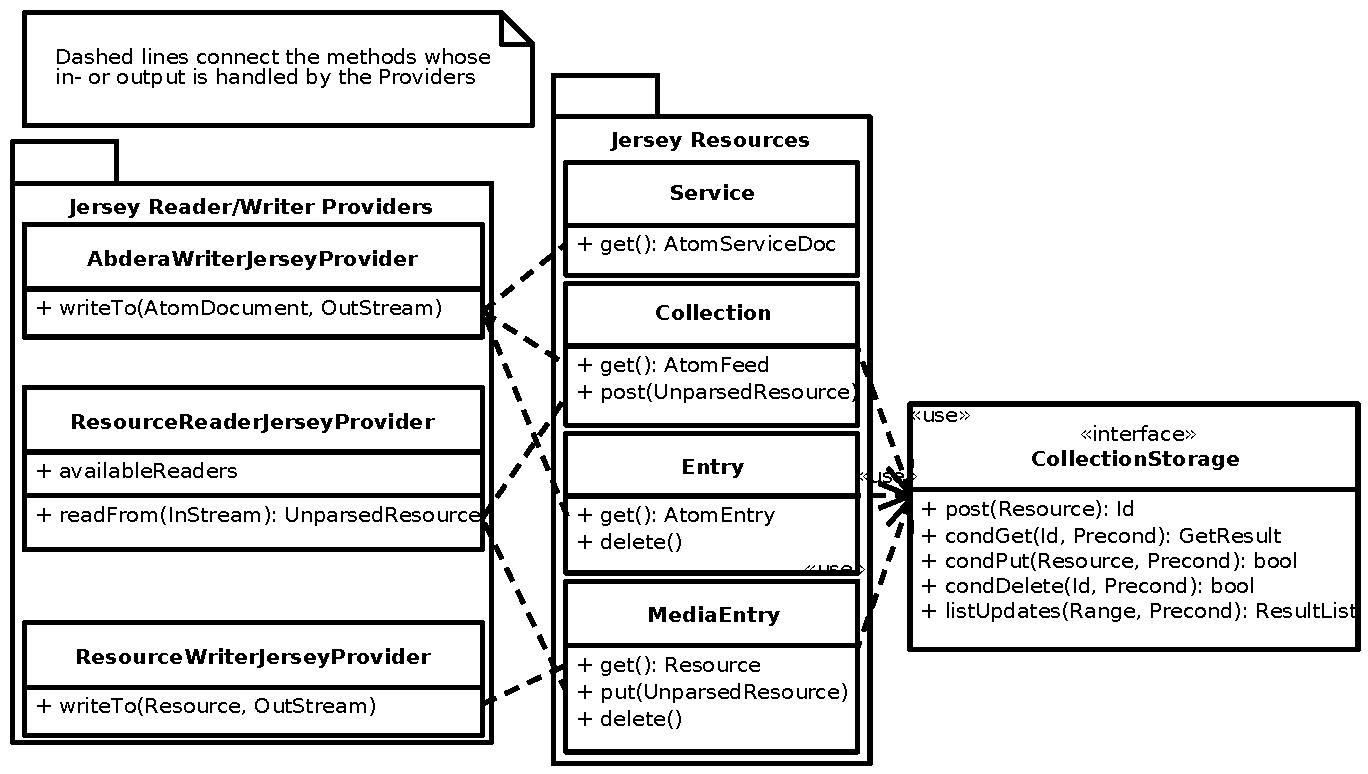
\includegraphics[width=1.2\textwidth]{executionflowoverview}

  \caption{main classes controlling the execution flow}
  \label{fig:executionflowoverview}
\end{figure}

\subsection{Resource handling}
\label{sec:resource-handling}

The \lstinline:Resource: class is the generalization of a RESTful HTTP resource
without a binding to a specific media type. This corresponds to the distinction
between a resource and its representations in Fielding's
Dissertation\cite[sec. 5.2.1.1]{Fielding2000}. A representation in a certain
format is a property ``selected dynamically based on the capabilities or desires of
the recipient and the nature of the
resource''\cite[p. 87]{Fielding2000}.

\subsubsection{Resource properties}
\label{sec:resource-properties}

The interface of the \lstinline:Resource: class marks the border between code
that handles the control flow of an HTTP request, as outlined in
\autoref{fig:executionflowoverview}, and code that provides information about
properties of a resource (\autoref{sec:resourcefacades}). In the context of this
work, four different kind of properties of resources are distinguished:

\begin{itemize}
\item essential administration properties: unique ID, last update time, HTTP
  entity tag
\item generic meta properties: title, summary, author
\item a media type independent interface corresponding to the concept represented
  by the resource, e.g., a person, location, event, product, \ldots
\item a media type specific serialization (representation) of the resource
\end{itemize}

The ID and update time are required for the synchronization protocol outlined in
\autoref{sec:interactions}. They do not depend on the nature or content of the
resource and are attached to the resource by code outside of the
\lstinline:Resource: class. The entity tag must differ for each new version of a
resource. The code to produce and check a resource's entity tag should be
adjusted carefully with the concrete CollectionStorage implementation to ensure
efficient processing of conditional HTTP requests.

The generic meta properties of the resource can be used to fill the
corresponding tags of an Atom entry. They can either be extracted from a
meaningful property of the resource or be provided to the resource. E.g., the
author property could be extracted from the meta data of an image file (EXIF) or
set to the organizer of an ical event. The title of a contact resource in the
implementation is set to its full name and email. The summary also contains the
address and phone number.

One use of two mediatype independent interfaces or ``facades'' or a resource is
exemplified in \autoref{fig:titleandsummary}. The \lstinline:Contact: interface
is implemented by two classes that can extract the necessary information from
either a \lstinline:VCard: or a \lstinline:PortableContact: instance. An
implementation of \lstinline:Contact: in turn is used by an implementation of
the \lstinline:TitleAndSummary: interface. The
\lstinline:PlainTextTitleAndSummary: class in comparison does not work on an
intermediary interface but directly on the original data structure.

The above mechanism is exposed by the \lstinline:getFacade(Interface): method of
the \lstinline:Resource: class and used to retrieve a
\lstinline:TitleAndSummary: facade in order to build an Atom Entry. The code
using the facade does not need any further knowledge about the type of resource
it is working with.

\begin{figure}[htb]
  \centering
  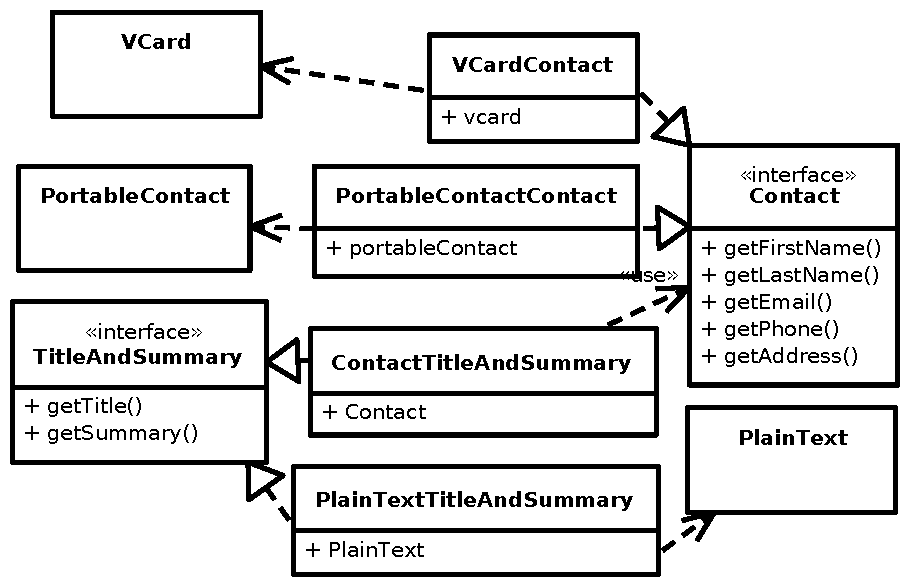
\includegraphics[width=1\textwidth]{titleandsummary}

  \caption{Dependency of facades of resources to provide the TitleAndSummary interface}
  \label{fig:titleandsummary}
\end{figure}

The serialization property is exposed by the asMediaType(MediaType,
OutputStream) method of the \lstinline:Resource: class. Internally this method
also uses the \lstinline:getFacade(): mechanism to request an instance of a
\lstinline:Writer: interface with the additional constraint that the writer must
produce the requested media type (\autoref{sec:resourcefacades}). Accordingly the
\lstinline:ResourceWriterJerseyProvider: of \autoref{fig:executionflowoverview}
is trivially simple: It just calls the asMediaType method of the provided
resource. The Resource is responsible for providing a media type specific
representation of itself.

The Resource class outlined in this section does not correspond to the equally
named resource class concept in JAX-RS \cite{JAX-RS1.1}. The latter kind of
resource classes are found in the ``Jersey Resources'' package of
\autoref{fig:executionflowoverview}. However such JAX-RS resource classes do not
really represent REST resources but rather the binding of resources to URIs and
their processing logic.

\subsubsection{Resource life cycle}
\label{sec:resource-life-cycle}

% @TODO visualisieren?

Resource classes in this work have a four staged life cycle. The first stage is
represented by the \lstinline:UnparsedResource: class, instantiated by the
ResourceReaderJerseyProvider class for post or put requests. In this stage, the
resource has already been assigned an appropriate \lstinline:Reader:
implementation according to the Content-Type request header but it has not yet
received an ID and update timestamp.

The \lstinline:Resource: class represents the second stage, a parsed request
body with an ID and update timestamp. Only in this stage the
\lstinline:getFacade(): method can be used.

Once a resource has been deleted, it does not vanish entirely, but enters stage
three. Only the associated data originally submitted in the request body is
discarded but the ID and update timestamp (now referring to the time of
deletion) is preserved. Such a ``deleted resource'' is used to generate a
corresponding ``deleted-entry'' tombstone in the AtomPub feed
(\autoref{sec:synchr-coll}).

Deleted resources don't need to be preserved eternally. A deleted resource with
the oldest timestamp of all resources managed by a particular CollectionStorage
can be safely purged completely (stage four). A client that synchronizes the
collection can still infer that the resource has been deleted since it is no
longer included anywhere in the list of updates. Repeated application of the
above rule makes sure that the last element of the updates list points to a
``living'' Resource of the second stage.

\subsubsection{Resource Facades}
\label{sec:resourcefacades}

Subsection \ref{sec:resource-properties} introduced and motivated the concept of
Resource Facades. This section explains the inner workings of the classes
providing this mechanism as drafted in \autoref{fig:resourcefacades}.

The Resource class does not hold any attribute that directly corresponds to its
``main'' or ``body'' data. Instead it holds a FacadeProvider instance to request
a specific data facade to access data. Facades are primarily referenced by Java
interfaces.

A FacadeProvider in turn is instantiated with a FacadeRegistry of available
FacadeFactories and one or more ``seed'' facades, making up the initial content
of the resolvedFacades attribute. An instance of FacadeFactory is capable of
building one specific facade object and has a set of dependencies needed for
that purpose. Therefor the concrete FacadeFactory used to build a facade and
thus the resulting implementation of the facade interface depends on the facades
already available in the resolvedFacades attribute of the FacadeProvider.

In the example of \autoref{fig:titleandsummary}, the TitleAndSummary interface
is implemented by two different classes. The factory responsible for the
PlainTextTitleAndSummary would declare a dependency on a PlainText facade. The
factory producing the ContactTitleAndSummary declares a dependency on a Contact
facade, which can again be produced by two different factories with their
dependencies finally pointing to the ``root'' facades.

Facades already resolved are added to the resolvedFacades attribute of the
FacadeProvider to speed up future facade requests. This is possible since
facades are required to only provide read access to the data. Any manipulation
of the Resource should result in a new Resource instance thus reflecting the
REST characteristic that Resources are manipulated by the submission of new
Representations.

Requests for facades can be further parameterized with a Predicate. The
Predicate has one \lstinline;apply(FacadeFactory):boolean; method which is
called only for FacadeFactories producing the desired interface. This mechanism
is used in the implementation to check an \lstinline:isWriteable(MediaType):
method on factories producing Writer instances and thus to select the correct
Writer according to the media type accepted by the client. Future work could
considerably enhance this rather brittle mechanism, e.g., to check for
annotations on the class produced by the factory.

\begin{figure}[htb]
  \centering
  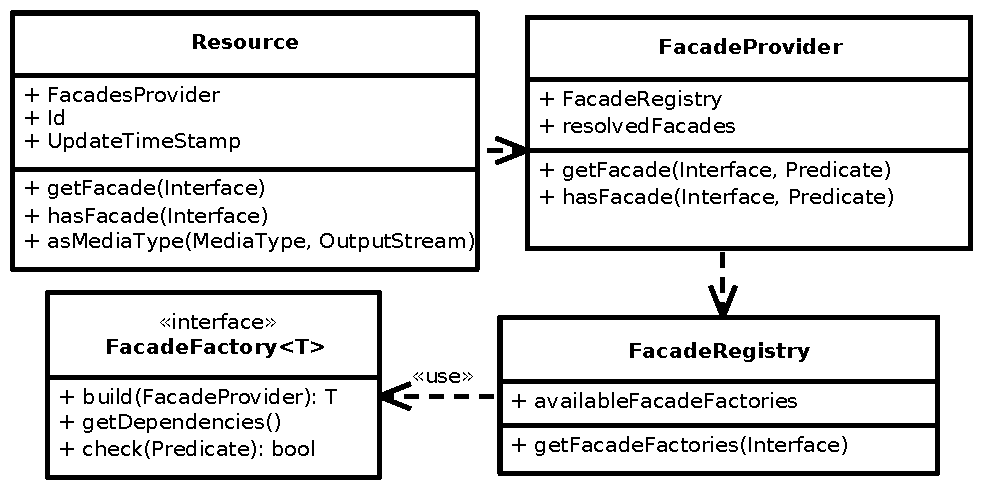
\includegraphics[width=1\textwidth]{resourcefacades}

  \caption{The API of the Resource Facades mechanism}
  \label{fig:resourcefacades}
\end{figure}

The Resource Facades concept is implemented only as a proof of
concept. \autoref{sec:resourcefacadesfuture-work} outlines a lot of future work
that might be worth consideration in this direction.

% A resource method should contain the programming logic executed to serve a
% request of a specific type (e.g., GET, PUT) against a specific resource. The
% programming logic could execute common tasks like the following:

% \begin{itemize}
% \item validate the correctness of a submitted resource
% \item check the client's authorization
% \item persist the submitted resource data
% \item trigger notifications containing a summary of the resource
% \item submit the submitted resource to an indexing system
% \item check the submitted resource to be of a certain accepted domain type, like
%   contact, event, to-do item or any set of such types
% \end{itemize}

% All the above processing tasks should in theory be independent of the media type
% of a resource and only be programmed once to work on any resource format. This
% could be made possible by applying the concept of roles to resources. Roles have
% been described already 15 years ago by \cite{Fowler1997} or a bit later by
% \cite{Baeumer2000}. However no evidence could be found whether roles have been
% used to implement RESTful systems.

% According to \cite{Steimann2008}, there exist several definitions for roles
% which mostly share a few core properties:

% \begin{quote}
%   This includes the property that a single object can play several roles of
%   different or the same kind both simultaneously and sequentially, and that the
%   same role can be played by different objects of the same and different
%   kinds. Raised to the type level, this means that the relationship between role
%   types and class types (as sources of role players) is generally m:n.
% \end{quote}

% A popular example for roles is a person that can have the different roles over
% their lifetime (student, professor, single, husband, widower) or in different
% contexts (teacher, father, husband, customer, politician).

% \cite{Steimann2001} repeats the necessity of the dynamic role concept and argues
% that (Java) interfaces serve as an appropriate means to handle roles.

% Exemplified with the above tasks, a resource can have the role of being
% validated, persisted, summarized or checked for being of a certain type. So like
% in the above quote a facility is needed that can provide m different roles of
% resources that come in n different shapes.

% It can be noted that unlike in the previous example with roles of a person,
% these resource roles examples do not extend the original resource with new
% attributes. A person surely gets additional attributes as a father (references
% to children) or professor (member of faculty). Thus the term ``facade'' in favor
% of role should indicate that only different views of the same data are provided.

% Listing \ref{fig:datafacades-api} shows interfaces of a minimal framework to
% provide Facades for Resources. The idea is that any code that needs information
% from a Resource requests the appropriate Facade from the ResourceHandler. The
% ResourceHandler was instantiated with a FacadeRegistry from which it can request
% Factories for requested Facades. A ResourceHandler must have been instantiated
% with at least one initial input Facade, e.g., an InputStream.

    % Facades provide read-only access to the data
    % Facades can depend on other Facades and thus reuse work
    % Facades could do:
    %     Parse the InputStream with a common JSON/XML framework
    %     Could check whether the data represents a concept like a contact or calendar item, independent from the underlying Media Type (vCard, xCard, portable contacts, iCal, xCal)
    %     Could provide a transformation to another representation (XML<->JSON, xCard to portable contacts)
    %     could extract generic informations from different media types: Title, Authors, Updated, Summary
    % A Facade (Java Interface) that provides access to the Name of a Contact Resource could be implemented by different classes that could work either on vCard, xCard or Portable Contacts. The resource method does not need to be aware or the original media type of the data.

% The concept is powerful because Facades can easily be added without changing
% existing classes. In JAX-RS the resource Method needs to decide which
% representation of the data it wants to work on. With this concept, a resource
% method could use several different available Facades to access the data.

% Using a similar concept to build representations (request Facades) for different MediaTypes may not be worth the effort.
% This would mostly be necessary to handle GET requests. GET requests however are expected to be idempotent and therefor should contain little to no internal side effects.
% It therefor seems to be reasonable to provide one GET request method for every produced Media Type.
% Specialized get requests may also execute faster than an approach that needs to dynamically build the processing pipeline.

% JAF + REST proposed in 2007 http://www.javaworld.com/javaworld/jw-10-2007/jw-10-resteasy.html

\subsection{CollectionStorage}
\label{sec:collectionstorage}

The CollectionStorage interface\footnote{The interface may be further broken
  down in a read-only and a write part which has been avoided for this
  overview.} is intended to be implementable for a variety of persistency
providers like relational databases, the file system, document databases like
CouchDB, MongoDB, eXist. In this context the IMAP folders used by Kolab are just
a kind of document store.

A CollectionStorage is instantiated with the knowledge of the collection for
which it is responsible. Each collection managed by the application corresponds
to a separate CollectionStorage instance. Several CollectionStorage instances
might however share the same underlying connection to a persistency provider.

The only uncommon requirement for the persistency provider is to provide the
time ordered list of updates. This list could be thought of as just another kind
of search or report like the full text and time range search defined by
OpenSearch (\autoref{sec:spec-reports-search}). A search index library like
Apache Lucene\footnote{\citeurl{http://lucene.apache.org}{2012-03-26}} can
provide indexes for full text search on text fields, time range on events or a
list of all documents ordered by an ``updated'' field.

The IMAP based persistency of Kolab does not provide the described
indexes\footnote{The IMAP SEARCH command\cite[sec 6.4.4]{RFC3501} searches only
  the message body and headers but not attachments.}. Those must therefor be
implemented by a separate component.

The CollectionStorage does not expose any support for transactions. This should
make the interface easier to implement and also corresponds to the REST
characteristics of statelessness and transfer of full representations. As a
consequence, the check for HTTP preconditions must be made inside the
CollectionStorage. Otherwise an update could be lost as demonstrated in Listing
\ref{fig:evaluatepreconditions-concurrency} from the JAX-RS
specification\cite[p. 28]{JAX-RS1.1}. In this example a concurrent update by a
separate HTTP request that would happen between the etag check and the
\lstinline:doUpdate: call would be overwritten.

\begin{javalisting}[label=fig:evaluatepreconditions-concurrency,
                   float=htb,
                   caption={Potential lost-update problem with JAX-RS}]
ResponseBuilder rb = request.evaluatePreconditions(etag);
if (rb == null) return doUpdate(foo);
\end{javalisting}

% a resource should not be build, it the etag has not changed. How to make
% etag checking as cheap as possible?

% Contactzilla.com saves portablecontacts json in MongoDB

%
https://groups.google.com/d/msg/portablecontacts/57R9gGyoqt0/-P0fF4zRjaoJ

\subsection{Dependency Injection}
\label{sec:dependency-injection}

% @TODO was einleitendes

\subsubsection{Preparsed Request Components with Dependency Injection}
\label{sec:prep-requ-comp}

It seems like an obvious fact that could not be further deduced that any
response action to a request must be preluded by a parsing of the request. In
the case of a REST application this parsing could be further divided in two
steps:
\begin{enumerate}
\item Parse URI, Accept Header and HTTP verb to select the Resource method
\item Resource method specific parsing defined by JAX-RS parameter annotations
  or performed in the Resource method
\end{enumerate}

JAX-RS defines only rudimentary support for the second step by means of
inflexible annotations. Listing \ref{fig:jaxrs-annotated-queryparams} shows as
an example the verbosity of parsing a set of standard query parameters for a
search interface.

\begin{javalisting}[label=fig:jaxrs-annotated-queryparams,
                   caption={Verbosity of parsing Requests with JAX-RS}]
@Get public Response get(
    @QueryParam("query") String query,
    @QueryParam("sort-by") String sortBy,
    @QueryParam("offset") int offset,
    @QueryParam("limit") int limit ) {
\end{javalisting}

The implementation for this work instead uses value objects\footnote{The ``value
  object'' design pattern describes immutable objects representing values. The
  equality of value objects depends only on represented value but not on object
  identity \cite[p. 486]{Fowler2002}.} and dependency injection to isolate
request parsing. This can be seen for example in the PaginationRange class which
should just hold the values of the URI query parameters limit and offset. The
provider function in Listing \ref{fig:paginationrangeprovider} is invoked by
Guice when this class is required. It depends in turn on UriInfo, extracts the
necessary information and returns a simple value object of the type
PaginationRange.

\begin{anylisting}[label=fig:paginationrangeprovider,
                   caption={Scala Dependency Injection provider for the PaginationRange class; intQueryParam extracts a named query parameter or returns the provided default value}]
@RequestScoped @Provides
def paginationRange(uriInfo:UriInfo):PaginationRange = {
  val queryParams = uriInfo getQueryParameters
  val offset = intQueryParam(queryParams, "offset", 0)
  val limit = intQueryParam(queryParams, "limit", 20)
  return new PaginationRange(offset, limit)
}
\end{anylisting}

Other similar value objects in the implementation provide injectable access to
the parsed path parameters (PathParam) or conditional request HTTP headers
(Preconditions). The main advantages of this approach are supposed to be:

\begin{itemize}
\item Classes that parse commonly used query parameters can be reused, even across
  unrelated applications.
\item The request method declaration becomes much easier to read.
\item Sophisticated validation can be applied without obfuscating the request method.
\item Value classes are the right place for additional logic related to the
  wrapped values. The Preconditions class for example contains the logic to
  check the If-* headers of a conditional request against the current entity tag
  or update time of a resource.
\item Default values for unspecified input could depend on information only
  available at runtime instead of being provided as static value to the
  applications source code.
\end{itemize}

%It is possible to implement this approach
% This approach is possible to implement for example with the dependency injection
% support provided by the Jersey
% framework.\footnote{\citeurl{http://codahale.com/what-makes-jersey-interesting-parameter-classes/}{2012-2-5},
%   \citeurl{http://codahale.com/what-makes-jersey-interesting-injection-providers/}{2012-2-5}}


\subsubsection{Driving Dependency Injection further}

The use of dependency injection can be extended to comprise several levels of
dependencies and thus to build processing pipelines.  The information from the
above PaginationRange class is in the implementation just forwarded to the
CollectionStorage's listUpdates method to receive a ResultList instance.

Consequently the resource method could as well use dependency injection to
directly request the required ResultList
instance. Figure \ref{fig:dependency-injection-pipeline} visualizes the resulting,
hypothetic dependency graph of this approach.

The figure shows how the CollectionStorage relevant for the request is
identified by the URI path. It depends of course on some kind of database.  The
dependency injection is configured to produce a ResultList class by calling the
listUpdates method of CollectionStorage with instances of PaginationRange and
Preconditions.

The idea might be an alternative implementation of processing pipelines to the
one proposed in \cite{Davis:2011:XTR:1967428.1967437}, which uses XProc, An XML
Pipeline Language. One advantage of the dependency injection approach would be
that the processing pipeline can be defined and configured in the same language
then the rest of the application.

\begin{figure}[tbp]
  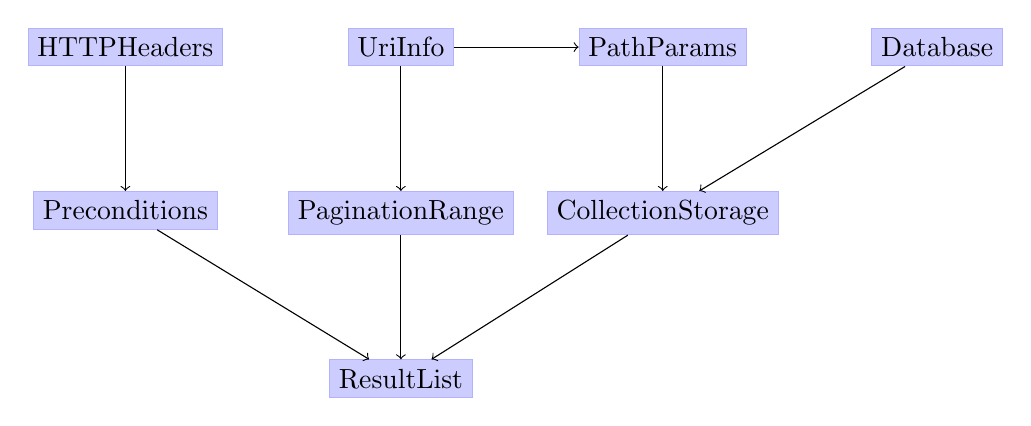
\begin{tikzpicture}
    [doc/.style={rectangle,draw=blue!30,fill=blue!20, node distance=4.5em}]

    \node[doc] (uriinfo) [] {UriInfo};

    \node[doc] (httpheaders) [left=of uriinfo] {HTTPHeaders};

    \node[doc] (Preconditions) [below=of httpheaders] {Preconditions}
      edge [<-] node [] {} (httpheaders);

    \node[doc] (PaginationRange) [below=of uriinfo] {PaginationRange}
      edge [<-] node [left] {} (uriinfo);

    \node[doc] (pathparams) [right=of uriinfo] {PathParams}
      edge [<-] node [above] {} (uriinfo);

    \node[doc] (database) [right=of pathparams] {Database};

    \node[doc] (collection) [below=of pathparams] {CollectionStorage}
      edge [<-] node [right] {} (database)
      edge [<-] node [right,text width=5em] {} (pathparams);

    \node[doc] (resultset) [below=of PaginationRange] {ResultList}
      edge [<-] node [left,text width=5em] {} (PaginationRange)
      edge [<-] node [right] {} (collection)
      edge [<-] node [] {} (Preconditions);
  \end{tikzpicture}
  \caption{Building a processing pipeline with Dependency Injection}
  \label{fig:dependency-injection-pipeline}
\end{figure}

\subsection{Routing and URI construction}
\label{sec:rout-uri-constr}

The normal way to bind JAX-RS resource classes to URI paths is provided by means
of the \lstinline:@Path: annotation. This has however several
disadvantages. First it hinders reuse of the resource classes in applications
with different URI paths. Furthermore it hinders the dynamic binding of new
paths to resources at runtime or the binding of methods from different classes
to the same path, e.g., to add additional HTTP method handlers. Finally all
definitions of paths are scattered throughout the code.

The implementation used the ``subresources'' feature of JAX-RS, which can help
at least to centralize the definition of URI paths in a \lstinline:Routes:
class. Methods of this class have \lstinline:@Path: annotations but no HTTP
method annotations. They don't handle the requests but instead instantiate and
return the appropriate JAX-RS resource classes which in turn have methods with
annotations for the supported HTTP methods.

The path templates themselves are static string members of the
\lstinline:Routes: class and thus also available for a \lstinline:LinkBuilder:
subclass of \lstinline:Routes:. The latter can be requested via dependency
injection and provides methods to construct links to all resources managed by
the system.

The centralization of routing and link building has one very important advantage
for REST applications. If such a central interface exists, than no other place
in the code, nor the public documentation should know which URIs are matched and
build by the interface. This would hopefully hinder all involved parties to
expect or document static URI patterns and instead force anybody to follow
hyperlinks.

The handling of URIs could have been implemented much more elegant by building
path templates dynamically at runtime. Unfortunately Jersey does only support
the static definition of paths at compile time thus only static strings could be
used for the definition. The upcoming version Jersey~2 however should provide
dynamic path
construction\footnote{\citeurl{http://java.net/jira/browse/JERSEY-842}{2012-2-6}}. Other frameworks, e.g.
Restlet\footnote{\citeurl{http://wiki.restlet.org/docs_2.1/13-restlet/27-restlet/326-restlet.html}{2012-2-6}} and
Apache Wink\footnote{called ``Dynamic Resources''
  \citeurl{http://incubator.apache.org/wink/1.1/html/5.1 Registration and Configuration.html}{2012-2-7}}
already have such a feature.

\subsection{Producing Semantically annotated HTML}
\label{sec:prod-semant-annot}

% @TODO das Problem wird nur bedingt klar, vor allem wenn man die Notation in
% Listing 7 und 8 nicht komplett kennt, aber es wird auf keinen Fall klar,
% welche Lösung du jetzt umsetzt

% XML transformations with scalate http://scalate.fusesource.org/documentation/scuery.html

A recent discussion of possibilities to produce semantically annotated HTML can
be found in \cite[sec. 9.1.3]{DBLP:books/daglib/0023755}. The authors describe a
method developed as part of a larger ``Web Semantics Design Method'' (WSDM),
which consists of two mappings. The first one is the ``data source mapping
(DSM), which describes exactly how the reference ontology maps to the actual
data source.''  The second mapping links HTML tags to elements of the reference
ontology from the first mapping. Neither the book nor referenced papers however
go into any more detail about the final step of generating the annotated HTML
tags.

One important point can be learned from the WSDM description. The production of
semantically annotated HTML can become a lot easier if the entity is already
available represented with the targeted vocabulary. A very naive approach to
produce annotated HTML would be to just manually write the necessary attributes
in the template and fill them with values from an arbitrary data object, as
demonstrated in listing \ref{fig:naive-microdata-template}. Even with the
conciseness of the used template language
Jade\footnote{\citeurl{http://scalate.fusesource.org/documentation/jade-syntax.html}{2012-2-22}
  Jade is the most concise among several supported template languages of the
  Scalate Template Engine.}, the developer still has a lot to type.

\begin{anylisting}[label=fig:naive-microdata-template,
                   caption={Defining all Microdata attributes manually in an HTML template}]
-@ var vcard: VCard

div( itemscope itemtype="http://schema.org/Person" 
     itemid=#{vcard.getProperty("uid")} )
  span( itemprop="name" )
    #{vcard.getProperty("fn")}
  span( itemprop="telephone" ) 
    #{vcard.getProperty("tel")}
\end{anylisting}

Compared to the above listing \ref{fig:microdata-template} shows a template
using a data structure that is aware of the used Microdata vocabulary and wraps
an instance of a typed Microdata item with its properties. The
\lstinline:scope: method of the Microdata interface will add the
\lstinline:itemscope:, \lstinline:itemtype: and \lstinline:itemid: attributes to
the nested \lstinline:div: element. The \lstinline:prop: method either augments
a nested element as shown for the \lstinline:name: property or creates the
correct nested element. The method adds the \lstinline:itemprop: attribute and
puts the value for this property inside the element.

\begin{anylisting}[label=fig:microdata-template,
                   caption={Using a Microdata-aware data structure in a template}]
-@ var md: MicroData

= md.scope
  div
    = md.prop("name")
      span( style="color:red" )
    = md.prop("telephone")
    = md.prop("email")
\end{anylisting}

An implementation of this approach must take care of a few
peculiarities \cite{Hickson2011}. Some properties don't necessarily use simple
\lstinline:span: elements, e.g., dates can be better expressed with
\lstinline:time: elements or URI values most likely appear in an
\lstinline:a:, \lstinline:img:, \lstinline:link: or \lstinline:object:
element. Property values could also be put in a \lstinline:content: attribute
while the element's nested text content is optimized for human
consumption. Items can be nested, e.g., an item of type PostalAddress could be
nested inside a Person item.

The proposed approach can be implemented on any template engine as long as it
permits to capture and manipulate nested HTML elements and to call methods of
passed in
objects.\footnote{\citeurl{https://github.com/Paxa/green_monkey}{2012-3-7}
  provides helpers to produce microdata in rails but is not as automated as the
  design proposed here.}


%\subsection{Reusability of Components}
%\label{sec:reus-comp}

% > - Wiederverwendbare Komponenten:
% >   - ResourceFacades Framework inkl. Medientypspezifische Klassen zur 
% > Extraktion,
% >     Transformation v. Daten
% >   - ATOM Framework (z.B. Abdera)
% >   - Extrem hilfreich: Dependency Injection
% >   - JAX-RS überraschenderweise wenig hilfreich
% >   - Einige kleine Helferklassen, die Funktionalität von JAX-RS ersetzen oder
% >     besser zugreifbar machen

% **** Zusammenfassung, Fazit

% > - Größtes Problem: Fehlende oder unzureichende Libraries zum Parsen, Bauen,
% >   Konvertieren der Medientypen. Erstellung und Pflege solcher Libraries ist 
% > eine
% >   langwierige Fleißarbeit.

\section{Results and Discussion}
\label{sec:results-discussion}

This section presents findings made while designing and implementing the
presented REST API, outlines which proposed goals have been achieved and why
others were not achieved, and proposes future work.

\subsection{Implemented Requirements}
\label{sec:impl-requ}

The implementation covers the provision of Atom Service Documents, Collections,
Entries and managed Media Entry Resources of arbitrary media types. Resources can
be created, read, updated and deleted with support for conditional requests. The
Atom Collections support the described synchronization mechanism.

The Resource Facades component provides a framework to process and serve
arbitrary media types if the necessary interfaces are implemented. The
implementation of those interfaces can usually be done in a few lines of code,
if an appropriate library for the parsing and serialization of the media type is
available.

Unfortunately no evidence of the existence of the necessary libraries could be
found. The only active and usable iCalendar and vCard library
iCal4J\footnote{\citeurl{http://wiki.modularity.net.au/ical4j}{2012-04-03}} does
not yet support the newest versions of those standards, especially not their XML
variants. For PortableContacts, two Java library projects were found,
JPoco\footnote{\citeurl{http://code.google.com/p/jpoco}{2012-03-30}} and
asmx-poco\footnote{\citeurl{http://code.google.com/p/asmx-poco}{2012-03-30}},
but both have not produced a release yet and appear abandoned since at least
2010.

The situation for Microdata support is even worse. A web developer seems to have
no other choice today then to manually write and fill the necessary HTML
attributes in an HTML template engine. An alternative, automated approach has
been proposed in \autoref{sec:prod-semant-annot} but the implementation of a
corresponding Java library was not possible in the scope of this work.

\subsection{Hypermedia support and prior knowledge of clients}
\label{sec:hyperm-supp-disc}

A main question of this work was, how a groupware API could be designed that
requires minimal prior knowledge by the client. Especially all resources should
be discoverable by following links with the exception of one initial service
URI.

Figure \ref{fig:discoverypaths} outlines the resources and their discovery paths
as discussed in this work. It can be seen, that all of them are reachable
following links from the Atom Service Document. Collections link to the next
partial collection, to their entries and are reachable from the Service
document. The OpenSearch Description document includes an URI template to
construct a link to a search result in Atom format containing links to
collection entries. Additional links are defined as part of the specific media
types managed by the collections, e.g., a link pointing to the calendar of an
xCard or another to a participant of an event. The edges pointing to xCard group
and media album are dashed, because the corresponding link relations are not yet
officially registered as discussed in section \ref{sec:vcards-soci-netw}.

\begin{figure}[tb]
  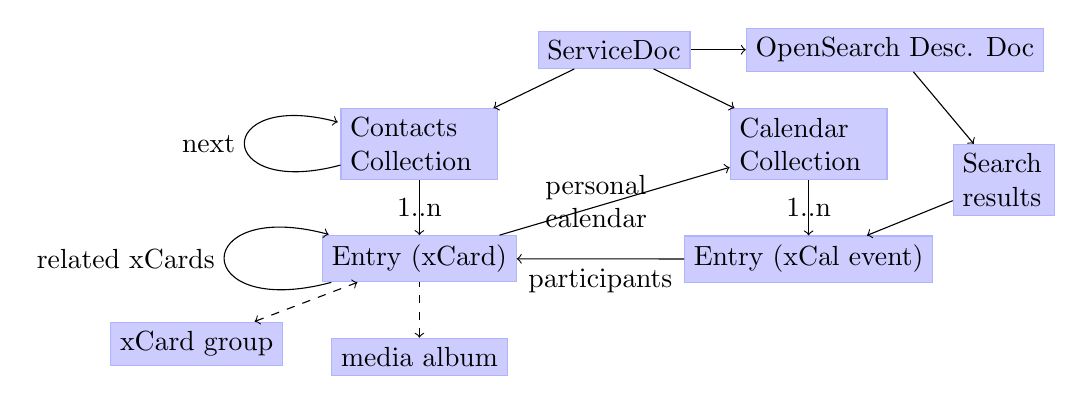
\begin{tikzpicture}
    [doc/.style={rectangle,draw=blue!30,fill=blue!20, node distance=1 em}]
    \node[doc] (svc) [] {ServiceDoc};
    \node[doc] (collect) [below left=2em of svc,text width=5em] {Contacts Collection}
      edge [<-] node {} (svc)
      edge [->, loop left] node {next} (collect);

    \node[doc] (calcollect) [below right=2em of svc,text width=5em] {Calendar Collection}
      edge [<-] node {} (svc);

    \node[doc] (opensearch) [right=2em of svc] {OpenSearch Desc. Doc}
      edge [<-] node {} (svc);

    \node[doc] (entry) [below=2em of collect] {Entry (xCard)}
      edge [<-] node {1..n} (collect)
      edge [->] node [text width=5em] {personal calendar} (calcollect)
      edge [->, loop left] node {related xCards} (entry);

    \node[doc] (event) [below=2em of calcollect] {Entry (xCal event)}
      edge [<-] node {1..n} (calcollect)
      edge [->] node [below] {participants} (entry);

    \node[doc] (searchresult) [above right=of event,text width=3em] {Search results}
      edge [->] node {} (event)
      edge [<-] node {} (opensearch);

    \node[doc] (group) [below left=2em of entry] {xCard group}
      edge [<->,style=dashed] node {} (entry);

    \node[doc] (album) [below=2em of entry] {media album}
      edge [<-,style=dashed] node {} (entry);
  \end{tikzpicture}
  \caption{Hypermedia links providing discovery paths from the Service Document
    to individual groupware resources}
  \label{fig:discoverypaths}
\end{figure}

All the above assumes, that the client has a built in understanding of the used
media types, i.e., Atom related types including the not yet standardized
deleted-entry, the OpenSearch Description Document and the types of the media
entries in this case xCard and xCal. Media entries may be available in
alternative representation enabling the client to negotiate the media type.

If semantic annotation (section~\ref{sec:microdata}) should be used then the
client also needs to understand the schema used for the annotations.

Necessary client knowledge that is not yet standardized but also not application
specific is:

\begin{itemize}
\item a link relation to the HTML form to create new entries (see
  section~\ref{sec:html-forms})
\item a schema providing atom categories to identify types of groupware
  collections (see section~\ref{sec:disc-coll})
\end{itemize}

\subsection{Media type libraries}
\label{sec:mediatype-libraries}

The support of REST for different media types has been blamed to potentially
``complicate and hinder the interoperability of a RESTful Web
service'' \cite[sec. 7.2]{Pautasso2008}. The experience made
in this work could not find any support for this assumption. It would of course
be preferable if all users of an API could be served and satisfied with the
same media type, but an API author may not be in such an advantageous
situation. The protocol related code in the server implementation however did
not become complicated even while serving and accepting arbitrary media types.

An area of immense complexity however is the parsing, serialization and
conversion of media types. This complexity exists every time when two
communication partners use different internal representations and must be solved
at some point between those partners. The REST API in this work imposes this
complexity on the server.

A symptom of the complexity involved with the handling of different media types
is the lack of stable or usable libraries. Contrasting to this there are dozens
of stable REST frameworks and libraries to choose from. It seems that the
development and maintenance of media type libraries is a neglected area.

In those libraries that exist and were used, some common shortcomings could be
observed that translate in the following advice for media type libraries:

\begin{itemize}
\item Unknown fields or properties should be preserved to support vendor
  extensions or updates in the specification.
\item Data structures should be immutable. The construction of the data
  structures should be delegated to separate, mutable Builders.
\item The scheme should not be hard coded in classes and their properties, but
  dynamically assembled at runtime. Cal4J, JPoco, asmx-poco or the OpenSocial
  implementation Apache Shindig all have one Java class for every known field.
  This requires many lines of unnecessary similar code and hinders extensibility
  and updates.
\end{itemize}

\subsection{Reusable Components}
\label{sec:reusable-components}

The main contribution of this work in terms of reusable components is the
concept and prototypical implementation of the Resource Facades. The proposed
design to support Microdata in template engines is also considered to be
reusable and beneficial for many use cases.

Surprisingly, the API of JAX-RS (or Jersey) was not as helpful as should be
expected from its official status. A couple of smaller classes were written for
this work to wrap Jersey's functionality and those should be reusable in
arbitrary REST projects. Some of those have been presented in
\autoref{sec:prep-requ-comp}: Preconditions, PathParams or PaginationRange. In
addition to this, a separate \lstinline:Routes: (\autoref{sec:rout-uri-constr})
class centralized the mapping from URI paths to resource classes, a
\lstinline:LinkBuilder: (ibid.) centralized construction of URIs and the reader
and writer provider classes delegated their work to the resource facades
framework. It seems advisable for further REST projects to evaluate frameworks
offering alternative concepts than JAX-RS.

% The main results of your work should be presented, together with critical
% discussion. The chapter should cover three things (although these would not be
% used as section headings):

% Findings. Present all the results (products, experimental findings, theories,
% etc.) generated during the project. This may also include some off-topic
% findings that were not expected, or which were side-effects of other
% explorations.

% Goals achieved. Describe the degree to which the findings support the original
% objectives laid out for the project. The goals may be partially or fully
% achieved, or exceeded. An experimental project may prove, or disprove the
% original thesis. A theoretical project may cover some or all of the example
% cases. Note that reporting of failures to achieve goals is important since a
% fundamental feature of the assessment procedures is that the processes (how you
% went about your project) are often as important as the products of the project.

% Further work. This should address two things: firstly, new areas of
% investigation prompted by developments in this project, and secondly parts of
% the current work which were not completed due to time constraints and/or
% problems encountered.

% further work
% establish full compatibility between PoCo and vCard/xCard and make it an IETF standard
% standardize feed diff http

% **** Hypermediabetrachtung in einen ganz eigenen Abschnitt eher gegen Ende der
% Arbeit, da könnte man zB super über (stark/schwach) zusammenhängende Graphen
% von Ressourcen/Medientypen reden

% Integrates nicely with other techniques: Pubsubhub, OpenID, OAuth

% Jersey, Guice, Guava, Abdera, ical4J, Scalate

%> - Auf Basis von Jersey, weil empfohlen von Schneider2010 (Vergleich und
%>   Beurteilung von Java Frameworks für Web Services mit REST)


\subsection{Future work}
\label{sec:further-work}

% @TODO einleitender Satz

% Apache Abdera 2 hat keine OpenSocial extension

% Abdera is nicht immutable

% XSL Stylesheets um HTML interface für ATOM zu bauen, z.B. von Google's Feedburner benutzt.

\subsubsection{Browser Caches as collection stores}
\label{sec:browser-caches-as}

The example of OpenSocial shows how important the browser has become as an
application platform. However browsers also restrict the options of developers,
especially in terms of available Webstorage (\autoref{sec:user-class-char}).

Clever use of the Browser cache could raise this limit. The average available
cache size is unknown but expected to exceed the web-storage size by several
orders of magnitude.

One interesting caching strategy in combination with collections is the use of
time based caching headers (\lstinline:expires: or \lstinline:Cache-Control:
with the \lstinline:max-age: directive) with long expiration times. The long
expiration time should keep the resource available even when the browser is
offline.

If the resource is updated, the long expiration time would normally prevent the
browser from updating it. However since the server controls the collection feed
linking to the resource, it can use a slightly different URI to link to the
resource on every update, thus forcing the client to do a reload. In this case
the client must have other means to keep track of the resource identiy: either
the ID element of the Atom Entry or a property of the resource itself, like the
UID property of vCard or iCal.

It would or course be even better, if Javascript code running in a browser could
somehow force a reload of a resource once it has learned from the collection
feed that the resource has been updated. In this context the exact caching
behavior of popular browsers is of interest, especially in combination with
Content-Location headers or the only-if-cached directive.

\subsubsection{Patching Resources}
\label{sec:patching-resources}

\autoref{sec:effic-synchr-with} introduced Delta Encoding \cite{RFC3229} and
mentioned that it would also be useful to efficiently respond to GET requests on
resources that only slightly changed (e.g., by one property field) compared to
the resource cached by the client.

The same argument applies for the other direction, if a client updates a large
resource. The HTTP PATCH method \cite{RFC5789} has been especially standardized
for this case in March 2010. Support for the PATCH method can be advertised in
the ``Allow'' header of server responses and the ``Accept-Patch'' header
specifies the media types of accepted patch formats.

However until today no patch format media types are listed in the official IANA
registry\footnote{\citeurl{http://www.iana.org/assignments/media-types/index.html}{2012-03-24}}
and a draft for a JSON patch format has
expired\footnote{\citeurl{https://datatracker.ietf.org/doc/draft-pbryan-json-patch}{2012-03-24}}.

More critical for this work is that no means have been foreseen to specify the
exact representation of a resource to which a PATCH should apply. So given a
server that can represent contacts in vCard, xCard and PortableContacts under
the same URI depending on the media type accepted by the client and a byte
oriented patch media type like the output of the unix \lstinline:diff -e:
command\footnote{\citeurl{http://www.iana.org/assignments/inst-man-values}{2012-03-24}}. How
should the server know against which format the patch should be applied?

At least three solutions may be possible:
\begin{itemize}
\item A different patch media type is used that is defined to apply to a specific
  representation. (This is recommended in \cite[ch. 11.9]{Allamaraju_2010}.)
\item The server uses separate URIs for different media type representations as
  suggested by \cite{Raman2006} and accepts PATCH request only against those
  URIs.
\item The server uses different entity tags for different representations that
  it can later use to parse the original resource media type from the etag
  supplied in the If-MAtch header of the PATCH request.
\end{itemize}

A further discussion of patch requests should also consider, whether this
request type still conforms to the REST interface constraint ``manipulation of
resources through representations''\cite[sec. 5.1.5]{Fielding2000}.

\subsubsection{JSON based media types for collections}
\label{sec:media-types-coll}

This work examined an API that can serve contact information in different
media types based on XML, JSON and RFC822. However it only considered one XML
based format for the discovery of those. It would be desirable to be able to
provide an API variant exclusively based on JSON. Therefor a JSON alternative
for the ATOM Publishing Protocol is needed.

\paragraph{Collection+JSON}
\label{sec:collection+json}

The Collection+JSON Mimetype (IANA registered in July 2011) by Mike
Amundsen \cite{Amundsen2011a}\cite[ch. 3]{amundsen2011building} looks like a
promising candidate for a JSON alternative. The author even states that is has
been explicitly designed after the model of the Atom Publishing
Protocol\footnote{\citeurl{http://amundsen.com/media-types/collection}{2012-03-22}}.

The media type defines a JSON structure which contains:

\begin{itemize}
\item query templates for the construction of query URIs
\item an array of collection items
\item one write template to create or edit items
\item meta data about the collection
\end{itemize}

Unfortunately, Collection+JSON in its current state is not yet fully usable to
implement the interactions described in \ref{sec:interactions}.

Collection+JSON does not enforce an order of the elements in a collection. The
proposed synchronization interaction however is based on the assumption that the
collection feed is ordered by the time of the last modification. Consequently,
there is also no equivalent to an ATOM
``deleted-entry'' \cite{draft-snell-atompub-tombstones-14}, which enables the use
of an updates feed for synchronization.
% @TODO wenn man entsprechende Filter anbietet ist die Sortierung nicht mehr unbedingt relevant

The facility to include full item representations directly in the collection
(the ``data'' property) is restricted to simple key/value pairs. This excludes
more complex data structures, like PortableContacts. It would still be possible
to omit the optional data property and only fill the href property with a link
to the full representation.

An AtomPub collection declares its accepted media types and assumes that the
client knows how to produce those. The Collection+JSON media type instead
provides a write template which the client must fill in order to create new
items. The write template only supports basic key value pairs in accordance to
the data property. More complex schemes can not be expressed\footnote{It would
  make sense to rely on JSON schemas to define valid item structures:
  \citeurl{http://json-schema.org}{2012-03-22}}.

A Collection+JSON document is furthermore restricted to contain only one write
template. This excludes mixed collections of different types.

Collection+JSON provides query templates but those come without a defined
semantic. A mapping from OpenSearch to JSON would be helpful to reuse the
semantic definitions. Also the URI template part should be updated to reuse the
specification of the new URI templates standard \cite{RFC6570}.

Pagination link relations for feeds \cite{RFC5005} could be reused to express
paginated JSON collections as encouraged by the format
documentation\cite[sec. 5.5]{Amundsen2011a}.

% 3.4. links "The links array is an OPTIONAL child property of the items array." and the collection!

\paragraph{Direct Mapping of ATOM XML to JSON}

James Snell described a mapping of ATOM XML to JSON that should not loose any
information \cite{Snell2008}\footnote{also implemented in Apache Abdera
  \citeurl{https://cwiki.apache.org/ABDERA/json-serialization.html}{2012-1-7}}. However
the attempt to map every feature of ATOM and the inherited extensibility and
expressiveness of XML results in a very complex and deeply nested JSON
structure. In detail, Snell identifies a couple of problems that need to be
dealt with in such a mapping \cite{Snell2008}:

\begin{itemize}
  \item JSON has no equivalent for the xml:lang attribute.
  \item Dereferencable IRIs must be transformed to URIs.
  \item URIs relative to an xml:base attribute must be resolved, also inside XHTML content elements.
  \item Repeatable elements must be converted to arrays.
  \item The ATOM date format (RFC 3339) differs from the JavaScript Date serialization.
  \item ATOM content elements are versatile but should be represented more meaningful in JSON then just a plain String.
  \item ATOM supports arbitrary extensions via namespaces.
\end{itemize}

Considering all the problems, it is understandable that no effort could be found
since 2008 to formalize the outlined mapping in an IANA registered media type.

\paragraph{Conclusion}

% Google's GDATA Json format, Youtube JSON feed?
Other related formats considered are the ``Hypertext Application Language''
(HAL) \cite{Kelly2011} and Microsoft's
OData\footnote{\citeurl{http://www.odata.org}{2012-03-23}}. HAL is a simple
container format that only standardizes linking and embedding of resources and
is rather meant as a building block or foundation for more specialized
formats. Collection+JSON as the more specialized format is therefor preferable
here.

OData shares many similarities with the Atom Publishing Protocol and also
provides a JSON variant of it. However, despite announcements in March
2010\footnote{\citeurl{http://web.archive.org/web/20110103120930/http://www.odata.org/blog/2010/3/16/welcome-to-the-new-odataorg!}{2012-03-23}},
Microsoft has not taken any steps so far to make OData an open standard that
could be safely used for free software projects.

In summary, the most promising approach for a JSON variant of ATOM seems to
enhance Collection+JSON in the following points:

\begin{itemize}
\item an indication, that a collection is ordered by modification time
\item means to indicate deletion of items
\item means to indicate accepted media types as an alternative to the write
  template
\item development and adoption of a JSON variant of OpenSearch
\end{itemize}

% http://code.google.com/apis/youtube/2.0/developers_guide_jsonc.html
% No replacement for Service document yet

\subsubsection{Push notifications}

This work does not include any means to actively notify (push) a client about
changes happening on the server. The client needs to initiate a request (pull)
to the server to look for changes. However separate solutions
exist\footnote{most notable PubSubHubBub \cite{Fitzpatrick2010}} to enable a push
  workflow on top of a feed based application
  \cite{Wilde:2009:FQP:1693155.1693220}. It may therefor not be seen as a
  disadvantage that push notifications have been omitted as a
  requirement.\footnote{\cite[sec. 1]{RFC6352} explicitly mentions missing
    ``change notifications'' as a ``key disadvantage'' of CardDAV.}

\subsubsection{Resource Facades}
\label{sec:resourcefacadesfuture-work}

The idea for the Resource Facades concept was triggered by the use of the
JavaBeans Activation Framework (JAF)\cite{Calder2006} in the JAX-RS
specification. In this framework the DataHandler interface provides access to
available commands for a specific MediaType via the getCommand method. The
framework however was designed with the needs of a Desktop clipboard in
mind. Since JAF has been released for Java version 1.4 it also does neither
support Generics nor uses the advantages of immutability.

\cite{Pradel2008a} presents an approach and implementation in Scala to attach
roles to arbitrary objects. The work achieves type safe roles without extending
the underlying language. Using this library has been considered but it was
discovered too late to be included. Open questions are how the declared media
type of a Resource could be considered in the selection of a role implementation
and how roles could depend on other roles. Another challenge would be to
preserve role instances and thus to avoid recreating them for every
invocation. If is furthermore required that roles implement a given
interface. The Resource Facade approach presented here is slightly different in
that creation of the facades is implemented independently from the facades
themselves by the factory classes.

% das Problem gehört meines Erachtens nach vorne wo du deine Lösung beschreibst und motivierst auch ein konkretes Beispiel, warum das bei dir keine gute Lösung ist wäre gut
JAX-RS provides the MessageBodyReader and -Writer interfaces. However these
interfaces are expected to be used only once per request. The resource method
afterwards needs to work with whatever interface was produced by the
MessageBodyReader. There exists no facility to request additional
transformations or facades of a Resource.

It is possible in JAX-RS to request a MessageBodyReader instance from the
\lstinline:Providers: interface. This couldn't however help to get additional
Facades since the InputStream has already been consumed.

The concept shows similarities with Dependency Injection since dependencies of a
facade are also provided by an external component. It may be possible that the
concept could even be implemented on top of an existing Dependency Injection
framework.\footnote{Scala can provide Dependency Injection solely with language
  features via the so called Cake Pattern \cite{Warski2011} \cite{Odersky2005}.}
 Some aspects however may require extra care:

\begin{itemize}
\item Resolving the dependencies of Facade factories must be parameterizable,
  e.g., to request a Writer instance for a specific media type.
\item The scope of an instance is bound to the ResourceHandler which in most
  cases may be equivalent to the Request scope, but this can't be guaranteed.
\item Each ResourceHandler manages its own view of available Facades.
\end{itemize}

The Apache Wink Rest Framework implements a concept called
``Assets''.\footnote{\citeurl{https://cwiki.apache.org/WINK/59-assets.html}{2012-2-28}}
Assets are containers for the resource data injected in or returned from
resource methods. Assets provide methods annotated with \lstinline:@Produces: or
\lstinline:@Consumes: to handle different Media types. In contrast to Resource
Facades, the set of supported media types of assets can only be extended by
extending the asset classes. It is also not possible like in
\autoref{fig:titleandsummary} to provide generic Facades for a TitleAndSummary
or Contact.

\paragraph{Scala's type system}

% @TODO ohne Scala Wissen nicht verständlich

 % @TODO Java class diagram?
The proposed Java class diagram in this section has the disadvantage that the
availability of a facade can not be checked at compilation time. It seems
however that a more advanced type system could help in this regard.

Listing \ref{fig:facades-with-scala-types} demonstrates features of the Scala
type system \cite{Odersky2011} that could be of interest here. In the example a
post method handler has the requirement to access the posted data through the
facades \lstinline:VCard: and \lstinline:TextSummary:. Additionally the data
should be forwarded to an implementation of the trait Storage which has its own
requirement for a facade.

Scala's ``compound types'' feature is used in line \ref{line-scala-compound} to
combine these requirements into an anonymous type. The ``type alias'' feature
allows it to assign the identifier \lstinline:MessageBody: to this anonymous
type and thus to keep the declaration of the \lstinline:post: method short and
readable.

\begin{javalisting}[label=fig:facades-with-scala-types,
                   numbers=left,
                   escapeinside={(*@}{@*)},
                   caption={Implementing the facades approach with Scala's type system}]
trait Storage[ReqFacade] {
 def create(id: String,
            body: ResourceHandler
                  with FacadeFactory[ReqFacade])
}

class PostToCollection[StorageReqFacade]
            (storage: Storage[StorageReqFacade]) {
 type MessageBody = ResourceHandler (*@\label{line-scala-compound}@*)
                    with FacadeFactory[VCard] 
                    with FacadeFactory[TextSummary]
                    with FacadeFactory[StorageReqFacade]
  
 def post(body:MessageBody) : Response = {
  ...
  storage.create("id", body)
  ...
 }
}
\end{javalisting}

This example and the mentioned work on Scala roles shows that an advanced type
systems may be able to considerably improve the presented facades approach. A
more detailed study however is out of the scope of this work and the author's
comprehension of type systems. % @TODO würde ich nicht schreiben?

\section{Conclusions}
\label{sec:conclusions}

% @TODO Check gegen Aufgabenstellung

% The conclusions can be summarised in a fairly short chapter (2 or 3 pages). This
% chapter brings together many of the points that you will have made in other
% chapters, especially in the previous results and discussion chapter. Do not be
% afraid of repeating some of your earlier statements here, albeit using different
% wording.

% Im Schlussteil sollen die wesentlichen Ergebnisse der Arbeit noch einmal herausgestellt werden.
% Dabei muss auf die eingangs formulierte Fragestellung eingegangen werden. Entweder kann die
% Frage nun beantwortet werden oder es ist darzulegen, warum sie nicht oder nur teilweise
% beantwortet werden kann. Im Schlussteil ist auch Kritik an der eigenen methodischen
% Vorgehensweise zu üben, insbesondere dann, wenn sie nicht die gewünschten Resultate geliefert
% hat. Aus dieser Kritik oder auch aus neuen Fragen, die bei der Bearbeitung des Themas
% aufgetaucht sind, sollte dann am Ende ein Ausblick auf die zukünftige Forschung hergeleitet
% werden.

It has been shown in this work that a rather uncomplicated, RESTful groupware
API is a usable alternative for more complex solutions like CardDAV or
OpenSocial. It even seems possible to serve the use cases of both protocols,
different classes of clients and different media type preference with the same,
unified, RESTful approach.

Most of the code necessary for the implementation is not even specific to a
groupware API but usable for other applications that offer a RESTful HTTP API
and might consume or produce multiple media types.

A great source of simplifcation and serendipitous reuse (e.g., VCards for social
network information, \autoref{sec:vcards-soci-netw}) is caused by the hypermedia
support of the involved media types.  The inclusion of complete, dereferenceable
URIs makes the need for verbose API documentations obsolete (like Opensocial,
\autoref{sec:opensocial-background}). The absence of hypermedia support, like
missing links to groups or albums in vCards, can directly constrain the possible
use cases of a media type.

Quite a few tremendously useful features of HTTP or the examined media types were
discovered during the research for this work, like HTTP delta encoding, Atom's
support for collection synchronization and categories or the versatility of
OpenSearch. Those were previously unknown to the author despite several years of
professional experience in web development. This supports the assumption that
lack of education might be a primary reason for the lack of REST adoption.

This work encountered complexities and lack of tooling in other areas then
expected. The initial research was spent on evaluating different platforms to
implement RESTful HTTP interactions. This area however proved to be rather easy
and well supported compared to the immense shortcomings or even lack of
media type libraries. This makes one wonder whether an expert group like
CalConnect should really work on additional protocols or rather on the problem
of lacking media type libraries.

\newpage
\bibliography{references}{}
\bibliographystyle{alphadin}

\end{document}

% Local Variables:
% ispell-dictionary: "american"
% eval: (progn (flyspell-mode 1) (outline-minor-mode 1) (goto-address-mode 1) (hide-body))
% End:
%  LocalWords:  RESTful programmatically instantiation hypothetic cacheable
% LocalWords:  Algermissen interoperability representable isomorphism doubtable
% LocalWords:  Cacheability extensibility referenceable shareable injectable
%  LocalWords:  dereferenceable mergeable unmergeable conformant parameterized
% LocalWords:  discoverable
